\documentclass{article}\usepackage[]{graphicx}\usepackage[]{color}
%% maxwidth is the original width if it is less than linewidth
%% otherwise use linewidth (to make sure the graphics do not exceed the margin)
\makeatletter
\def\maxwidth{ %
  \ifdim\Gin@nat@width>\linewidth
    \linewidth
  \else
    \Gin@nat@width
  \fi
}
\makeatother

\definecolor{fgcolor}{rgb}{0.345, 0.345, 0.345}
\newcommand{\hlnum}[1]{\textcolor[rgb]{0.686,0.059,0.569}{#1}}%
\newcommand{\hlstr}[1]{\textcolor[rgb]{0.192,0.494,0.8}{#1}}%
\newcommand{\hlcom}[1]{\textcolor[rgb]{0.678,0.584,0.686}{\textit{#1}}}%
\newcommand{\hlopt}[1]{\textcolor[rgb]{0,0,0}{#1}}%
\newcommand{\hlstd}[1]{\textcolor[rgb]{0.345,0.345,0.345}{#1}}%
\newcommand{\hlkwa}[1]{\textcolor[rgb]{0.161,0.373,0.58}{\textbf{#1}}}%
\newcommand{\hlkwb}[1]{\textcolor[rgb]{0.69,0.353,0.396}{#1}}%
\newcommand{\hlkwc}[1]{\textcolor[rgb]{0.333,0.667,0.333}{#1}}%
\newcommand{\hlkwd}[1]{\textcolor[rgb]{0.737,0.353,0.396}{\textbf{#1}}}%
\let\hlipl\hlkwb

\usepackage{framed}
\makeatletter
\newenvironment{kframe}{%
 \def\at@end@of@kframe{}%
 \ifinner\ifhmode%
  \def\at@end@of@kframe{\end{minipage}}%
  \begin{minipage}{\columnwidth}%
 \fi\fi%
 \def\FrameCommand##1{\hskip\@totalleftmargin \hskip-\fboxsep
 \colorbox{shadecolor}{##1}\hskip-\fboxsep
     % There is no \\@totalrightmargin, so:
     \hskip-\linewidth \hskip-\@totalleftmargin \hskip\columnwidth}%
 \MakeFramed {\advance\hsize-\width
   \@totalleftmargin\z@ \linewidth\hsize
   \@setminipage}}%
 {\par\unskip\endMakeFramed%
 \at@end@of@kframe}
\makeatother

\definecolor{shadecolor}{rgb}{.97, .97, .97}
\definecolor{messagecolor}{rgb}{0, 0, 0}
\definecolor{warningcolor}{rgb}{1, 0, 1}
\definecolor{errorcolor}{rgb}{1, 0, 0}
\newenvironment{knitrout}{}{} % an empty environment to be redefined in TeX

\usepackage{alltt}

%%% file preamble
\usepackage[utf8]{inputenc}       % Enable utf8 for input encoding
\usepackage[english]{babel}       % Enable English language for document
\usepackage{comment}              % Enable comments for paper
\usepackage{float}                % Enable 'H' for hard figure placement
\usepackage{fullpage}             % Enable fullpage specifications
\usepackage{amsmath}              % Enable math mode accessories
\usepackage{amsfonts}
\usepackage{amsthm}
\usepackage{amssymb}
\usepackage{bm}                   % Enable \bm{} for bold in math mode
\usepackage{graphics}             % Enable specific figure alignment
\usepackage{indentfirst}          % Enable indentation for all paragraphs 
\usepackage{subfig}               % Enable usage of sub-figures
\usepackage{hyperref}             % Enable usage of hyper-link references
\usepackage{textcomp}             % Enable usage of Trademark symbol
\usepackage{array}                % Enable usage for fixing table sizes
%\usepackage{hyperref}             % Enable usage of hyperlinks
\usepackage{fullpage}
\usepackage{pdflscape}

\hypersetup{
    colorlinks=true,
    linkcolor=blue,
    filecolor=blue,      
    urlcolor=blue,
}

\allowdisplaybreaks
%\setlength\parindent{0pt}



\title{Time Series Analysis on London Mortality}
\author{Egan McClave, Aijin Wang}
\IfFileExists{upquote.sty}{\usepackage{upquote}}{}
\begin{document}
\maketitle

\tableofcontents
\newpage

\listoffigures
\listoftables
\newpage

\clearpage
\setcounter{page}{1}

\begin{abstract}
\addcontentsline{toc}{section}{Abstract}

The purpose of this report is to examine and understand the relationship between the number of deaths and environmental variables such as particulate matter and some weather variables. We analyzed 4 time series with 1826 observations per each series. We fit several models (Time Series Regression, Vector autoregression, Neural Network rutoregression) in an attempt to estimate the health risks associated with the given environmental variables. Based on these different models, Temperature appears to have a very influential relationship on understanding the number of deaths.
\end{abstract}

\section{Introduction} \label{s:introduction}

Understanding mortality rates is an essential part of environmental epidemiology. Individually, ambient temperature/humidity and air pollution have been important determinants of mortality. It is of interest of us to investigate the associations between exposures such as air pollution, weather variables and human health. In this paper, we attempt to estimate the health risks associated with exposure to particulate matter (PM) and weather variables. Some advanced statistical models are necessary to study the possibly non-linear relationship among these variables of interest.

The data was originally introduced in the paper \textit{Time Series Regression Studies in Environmental Epidemiology} published in International Journal of Epidemiology. The paper can be found \href{https://www.ncbi.nlm.nih.gov/pmc/articles/PMC3780998/}{here}. The aim of the paper was to explore the basic modeling techniques that were appropriate for this problem. The data can be accessed from \url{https://www.ncbi.nlm.nih.gov/pmc/articles/PMC3780998/}. We will conduct our own analysis for this dataset and compare said results to the existing ones from the academic paper.

\section{Methods} \label{s:methods}
\subsection{Data Description}

The dataset contains daily observations of Ozone, O$_3$ ($\mu g / m^3$), Temperature ($^{\circ}$C), Relative Humidity (\%) and number of deaths from January 2002 to December 2006. A brief quantitative summary of the data is described in~\autoref{tab:data_summary}.

% latex table generated in R 3.4.3 by xtable 1.8-3 package
% Sun Apr 28 23:56:25 2019
\begin{table}[ht]
\centering
\begin{tabular}{rrrrrrr}
  \hline
 & Min. & 1st Qu. & Median & Mean & 3rd Qu. & Max. \\ 
  \hline
Ozone & 1.18 & 21.09 & 34.92 & 34.77 & 46.73 & 119.25 \\ 
  Temperature & -1.40 & 7.51 & 11.47 & 11.72 & 16.20 & 28.17 \\ 
  Relative Humidity & 31.23 & 58.69 & 69.61 & 69.10 & 80.36 & 98.86 \\ 
  Num Deaths & 99.00 & 135.00 & 148.00 & 149.51 & 162.00 & 280.00 \\ 
   \hline
\end{tabular}
\caption{Summary Statistics for Individual Time Series} 
\label{tab:data_summary}
\end{table}


\subsection{Exploratory Data Analysis} \label{ssec:EDA}
\subsubsection{Univariate EDA}

Before fitting time series models, we first want to understand the possible relationships among variables to get a better understanding about the structure of the data.

\autoref{fig:overall} shows the individual time series plots for the dataset. From \autoref{fig:overall} (a), we see that all three independent variables and the response variables have constant mean and variance. For number of deaths, there is an observation in 2003 that is extremely higher than the rest of the data. News reported that in August 3, 2003, Britain has recorded the highest temperature in 130 years, and the unusual weather might have led to the increasing number of deaths. Furthermore, the plots also suggests some seasonality effect in the data, since the plots show periodic patterns. Therefore, we explore the patterns by looking into the decomposed time series plots. 

\autoref{fig:overall} (b) displays the decomposed seasonality components for each series. As suggested in the overall series plot, we see an approximate yearly seasonality effect for all the variables. Specifically, \texttt{Ozone} and \texttt{Temperature} move in phase with one another as do \texttt{Num Deaths} and \texttt{Relative Humidity} with each other. However, these two pairings are out of phase with the other pair (they all have the same frequency $\approx$365 but change over time differently). We will consider seasonality in the model fitting.

\begin{knitrout}
\definecolor{shadecolor}{rgb}{0.969, 0.969, 0.969}\color{fgcolor}\begin{figure}[H]

{\centering \subfloat[Overall Series\label{fig:overall1}]{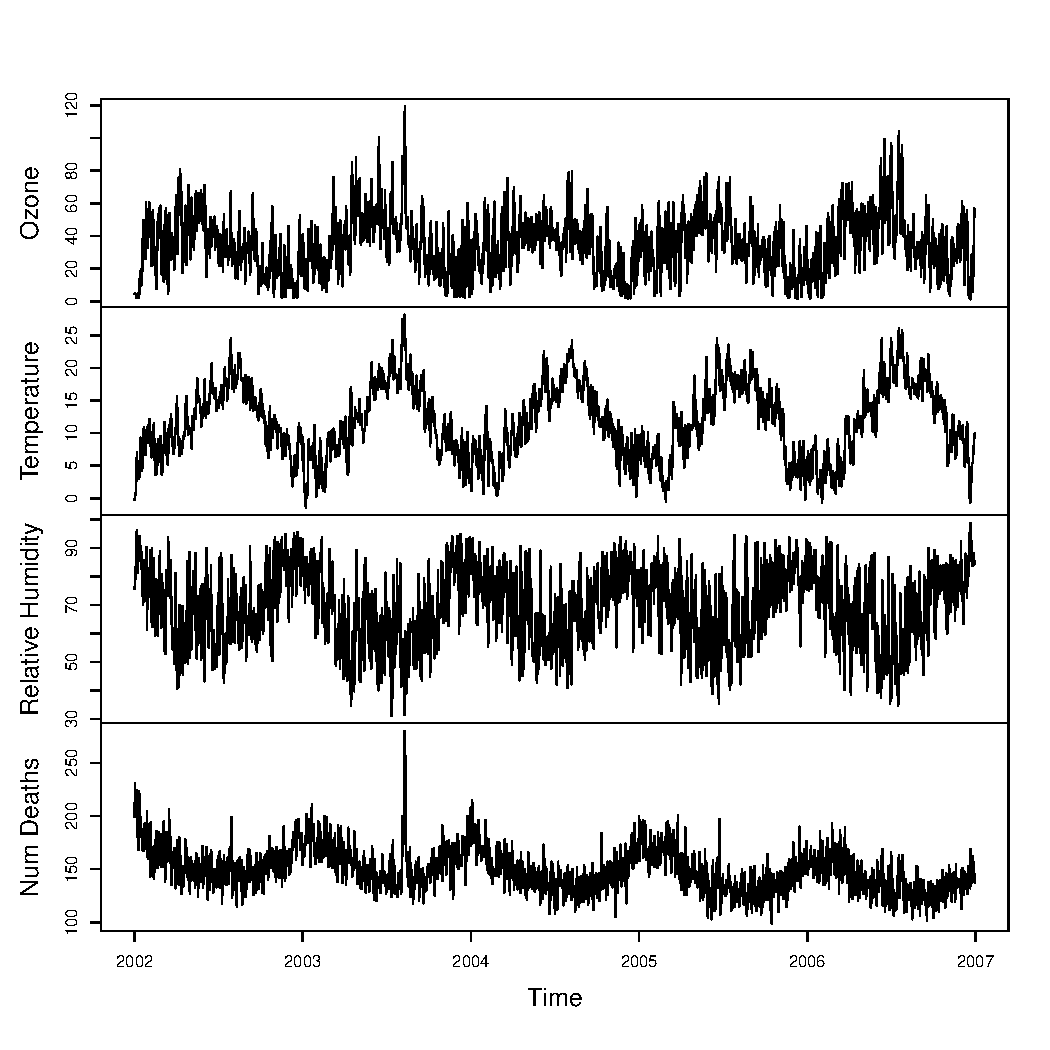
\includegraphics[width=0.45\textwidth]{figure/overall-1} }
\subfloat[Decomposed Seasonality Component\label{fig:overall2}]{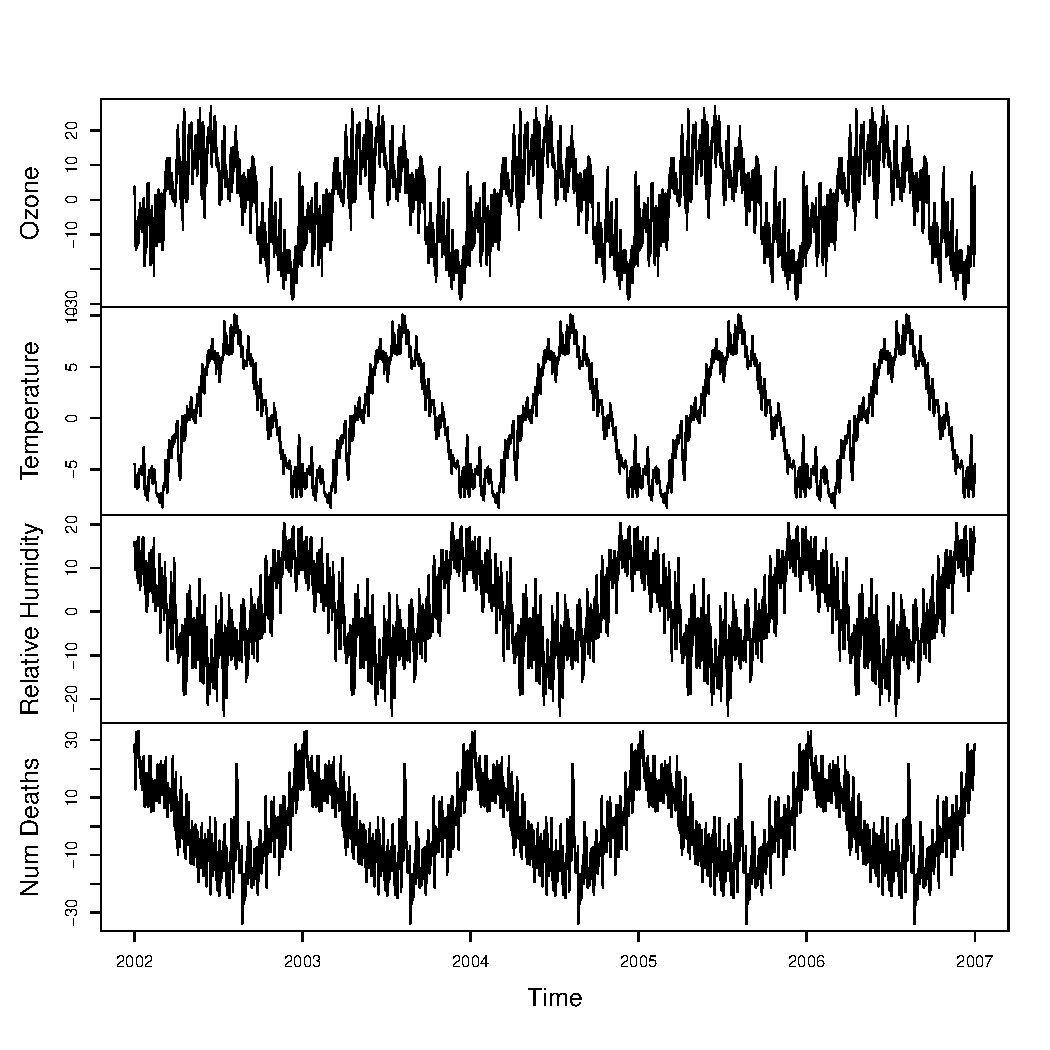
\includegraphics[width=0.45\textwidth]{figure/overall-2} }

}

\caption[Visualizing Individual Time Series for London (2002 - 2007)]{Visualizing Individual Time Series for London (2002 - 2007)}\label{fig:overall}
\end{figure}


\end{knitrout}

\subsubsection{Multivariate EDA}
\vspace{-20 pt}

\begin{knitrout}
\definecolor{shadecolor}{rgb}{0.969, 0.969, 0.969}\color{fgcolor}\begin{figure}[H]

{\centering 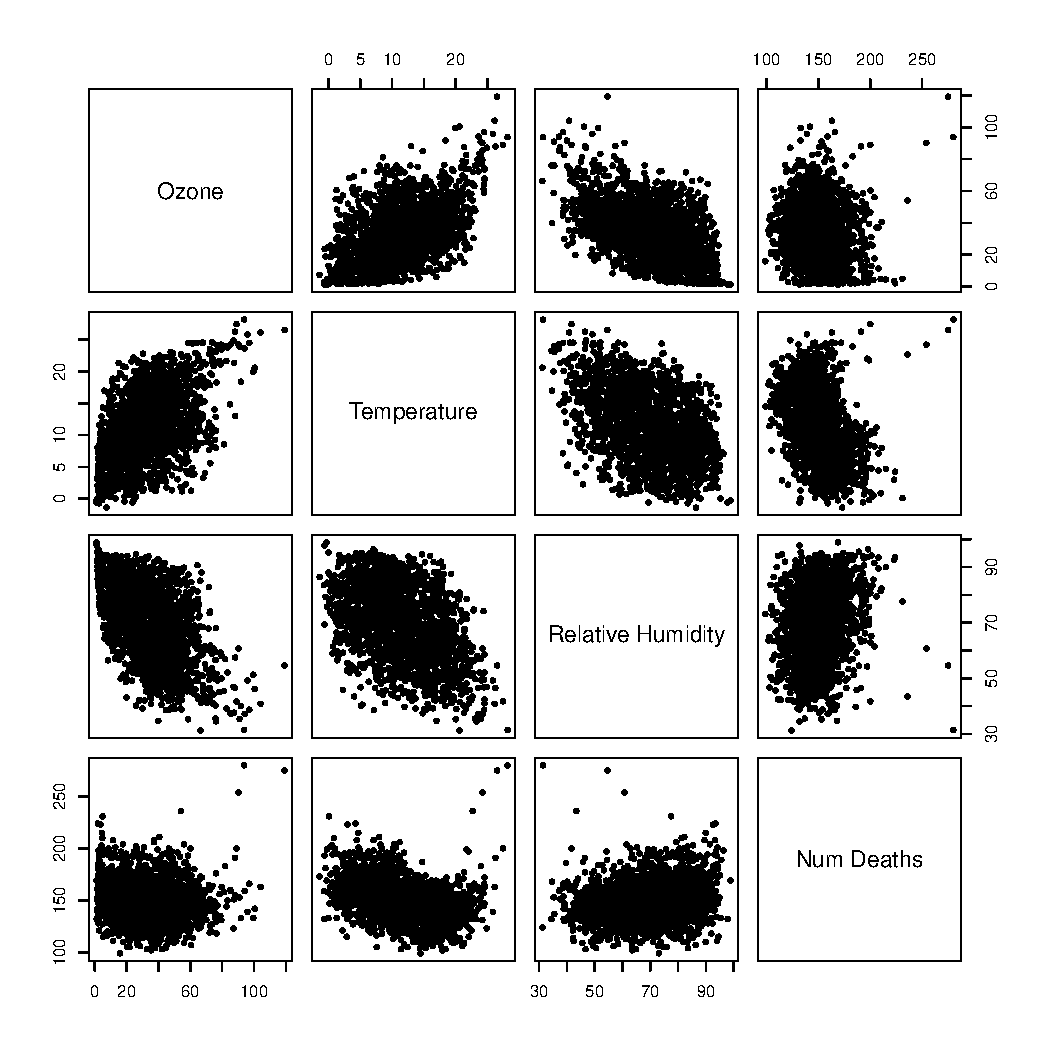
\includegraphics[width=0.55\textwidth]{figure/pairs-1} 

}

\caption[Pairs Plot of all Variables]{Pairs Plot of all Variables}\label{fig:pairs}
\end{figure}


\end{knitrout}

\autoref{fig:pairs} shows the pairwise scatterplots in the dataset. Both \texttt{Ozone} and \texttt{Relative Humidity} don't show strong correlation with \texttt{Num Deaths}, but there is a weak quadratic relationship between \texttt{Temperature} and \texttt{Num Deaths}. This suggests that some variable transformations may be useful in order to account for the relationship. 

\newpage
\begin{landscape}
\begin{knitrout}
\definecolor{shadecolor}{rgb}{0.969, 0.969, 0.969}\color{fgcolor}\begin{figure}[H]

{\centering \subfloat[ACF/CCF Plots of Individual Series\label{fig:cf_plot1}]{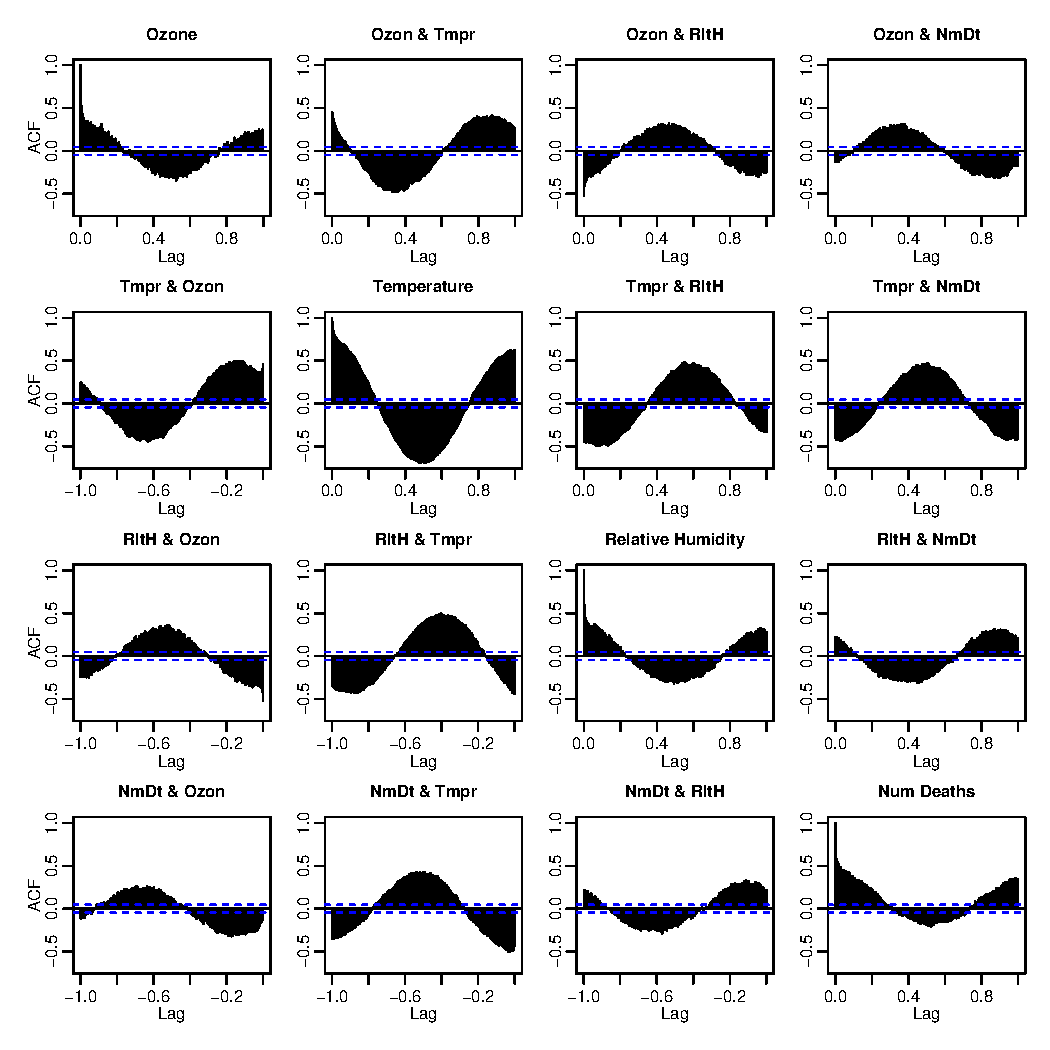
\includegraphics[width=0.70\textwidth]{figure/cf_plot-1} }
\subfloat[PACF/PCCF Plots of Individual Series\label{fig:cf_plot2}]{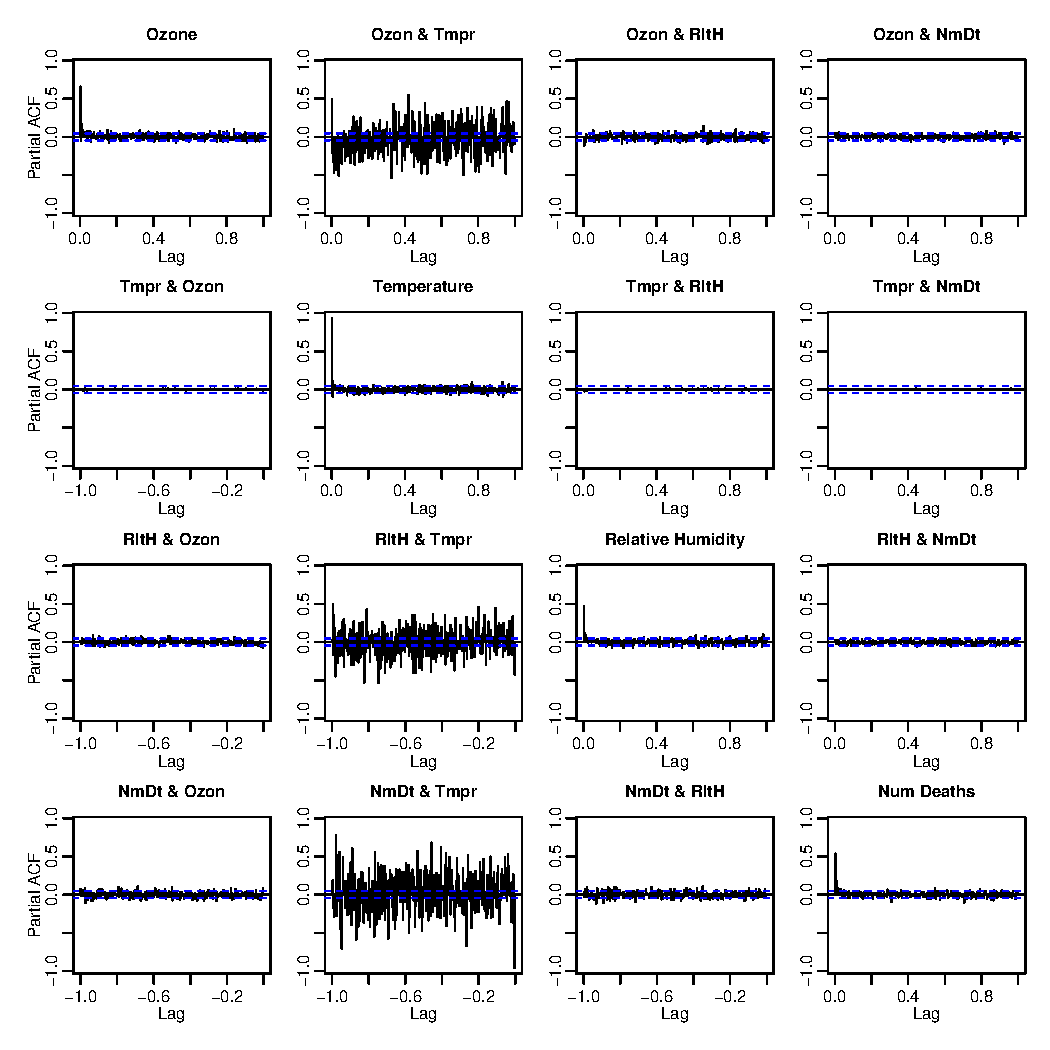
\includegraphics[width=0.70\textwidth]{figure/cf_plot-2} }

}

\caption[Auto-Correlation Plots of Individual Series]{Auto-Correlation Plots of Individual Series}\label{fig:cf_plot}
\end{figure}


\end{knitrout}

\autoref{fig:cf_plot} illustrate the ACF/CCF and PACF/PCCF of the individual series up to a full 365 days of lag. The ACF/CCF plots in~\autoref{fig:cf_plot} (a) that ACF values depend on the lag and have periodic patterns. Large number of the values are also outside the confidence level. This further proves that the original series is not stationary and have seasonality effects. 

There are four PACF plots on the diagonal as shown in~\autoref{fig:cf_plot}(b). For all four variables, the plots have tails off, meaning that some AR models are appropriate for the dataset. Out of all the PCCF plots, only the one between number of deaths and temperature has high PCCF values for various lags. This is evidence to prove that there might be some relationship between the two variables.
\end{landscape}

\subsection{Variable Transformation}

Based on the exploratory data analysis in~\autoref{ssec:EDA}, we discovered that there is potentially a quadratic relationship between \texttt{Temperature} and \texttt{Num Deaths}. Therefore, we will include a quadratic transformation of \texttt{Temperature} in the modeling. Furthermore, we use the mean adjusted version of \texttt{Temperature} instead of the original version to ensure the calculations are more stable. In addition, we also engineer the variables \texttt{Day of Week} and \texttt{Day of Month} from the dates provided.

In summary, below are the variables that we use for the model building after transformation:
\begin{itemize}
    \item \texttt{Time}
    \item \texttt{Ozone Levels}
    \item \texttt{Relative Humidity}
    \item \texttt{Adjusted Temperature}
    \item \texttt{Adjusted Temperature}$^2$
    \item \texttt{Num Deaths}
    \item \texttt{Day of Week}
    \item \texttt{Day of Month}
\end{itemize}



\subsection{Model Identification}
Based on the above analysis and the research goal of the project, we will be fitting three types of model, which are:
\begin{itemize}
    \item Time Series Regression
    \item Vector Autoregression
    \item Neural Network Autoregression
\end{itemize}

In this section, we will discuss the steps that we take to fit each model. 

\subsubsection{Time Series Regression}
\noindent\textbf{Manual Identification} \\

We first fit a simple linear regression model using OLS with all the variables mentioned above as exogenous variables. The residual plot, Q-Q plot, ACF and PACF of the residuals are displayed in \autoref{fig:ts_1} and \autoref{fig:ts_2}. The residuals in \autoref{fig:ts_1}(a) are not randomly distributed, and show some periodic patterns. Though the plot has mean centered around zero, it also shows heteroskedasticity. There are also four observations that have relatively high values. The Q-Q plot shows a similar result. The points show a bell curve, with the end of the plot being heavily tailed. These are evidence implying that the simple OLS model may not be a good fit for the dataset. 

The ACF and PACF plots prove that the residuals are not white noise, but instead have some AR and MA behavior. Upon further examination of the plots, we identify an \texttt{ARMA(2,8)} model for the residuals, and refit time series regression with all the exogenous variables assuming that the residuals follow ARMA with the orders (2,8) found in the previous step.

\begin{knitrout}
\definecolor{shadecolor}{rgb}{0.969, 0.969, 0.969}\color{fgcolor}\begin{figure}[H]

{\centering \subfloat[Residuals over Time\label{fig:ts_11}]{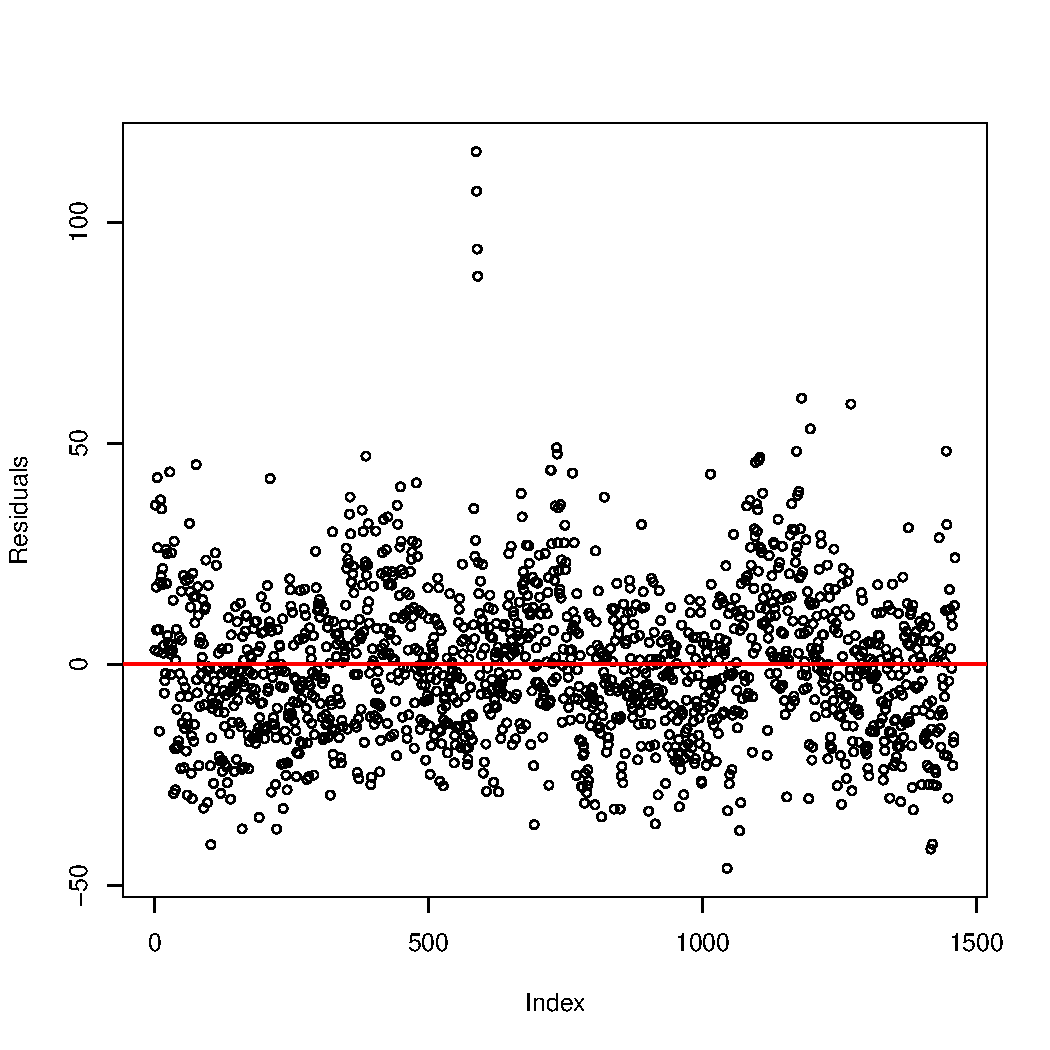
\includegraphics[width=0.50\textwidth]{figure/ts_1-1} }
\subfloat[Residual QQ Plot\label{fig:ts_12}]{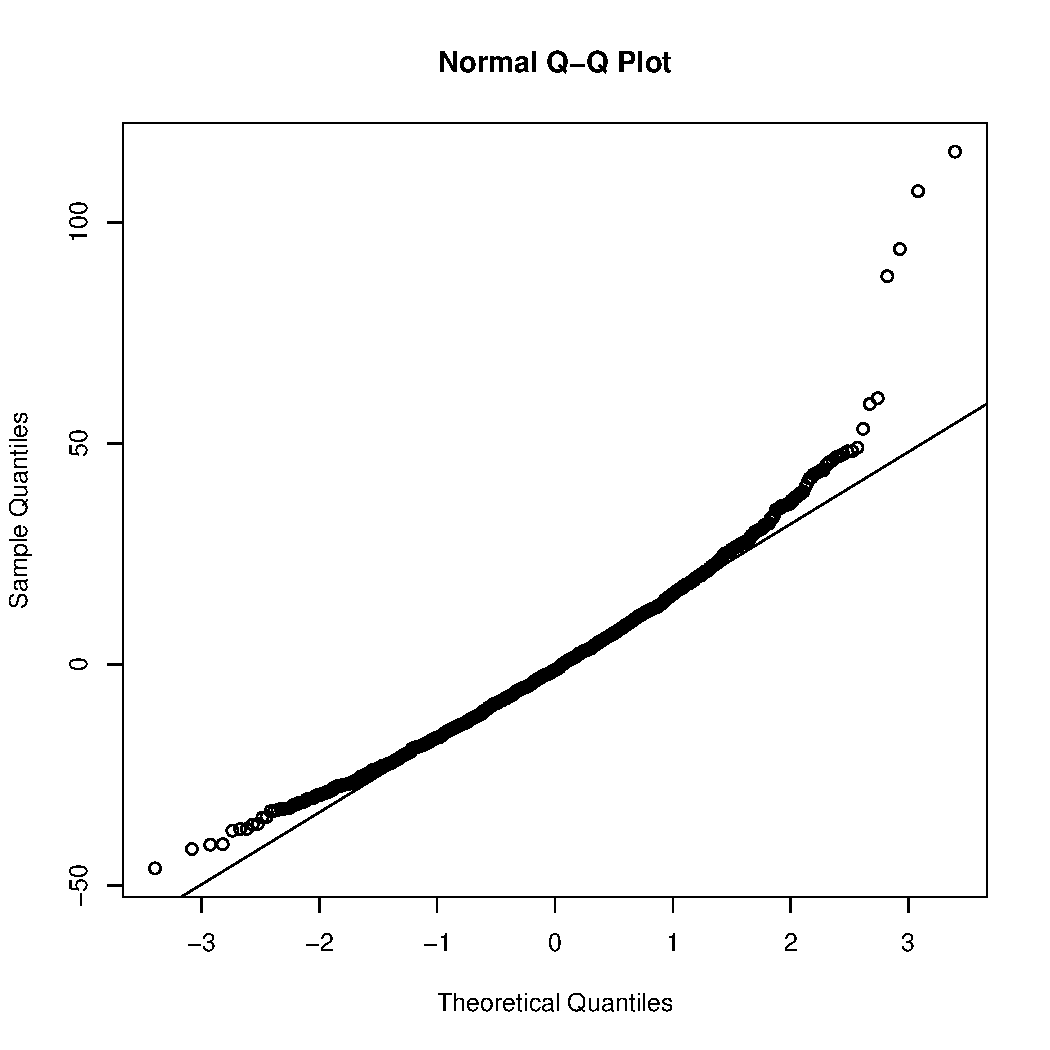
\includegraphics[width=0.50\textwidth]{figure/ts_1-2} }

}

\caption[Visualizing Residuals]{Visualizing Residuals}\label{fig:ts_1}
\end{figure}


\end{knitrout}

\begin{knitrout}
\definecolor{shadecolor}{rgb}{0.969, 0.969, 0.969}\color{fgcolor}\begin{figure}[H]

{\centering 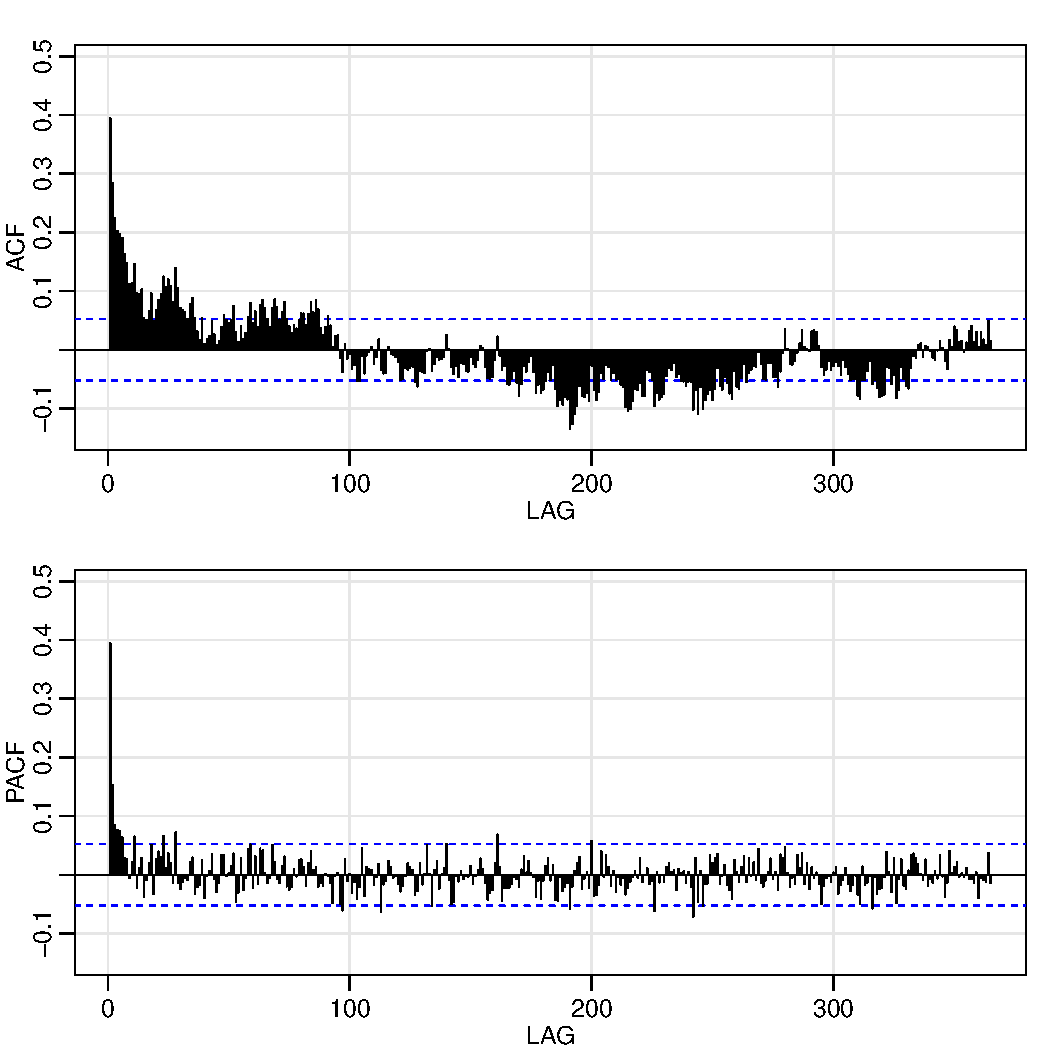
\includegraphics[width=0.65\textwidth]{figure/ts_2-1} 

}

\caption[ACF/PACF Plot of Residuals]{ACF/PACF Plot of Residuals}\label{fig:ts_2}
\end{figure}


\end{knitrout}

\noindent\textbf{auto.arima} \\
Another approach that can help identify the order of residuals is the function \texttt{auto.arima} in R. Since we already know that the residuals are not white noise, we will use \texttt{auto.arima}, which returns the best ARIMA model based on information criteria(AIC or BIC value) to get the order for the residuals. We will also be accounting for the effects of exogenous variables, same as the previous section. 

\begin{equation*}
    \texttt{model <- auto.arima(`Num Deaths', seasonal=T, xreg=\ldots, stepwise=F, approx=F, type=`none')}
\end{equation*}

After running \texttt{auto.arima}, we identidy an \texttt{ARMA(1,1)} model for the residuals. Same as above, we then refit time series regression all the exogenous variables, but assuming that the residuals follow ARMA with the orders (1,1).\\

The specific model fitting, validation and inference will be expanded upon in detail in~\autoref{ssec:ts_reg}. We will compare the results between ARMA(1,1) and ARMA(2,8) and identify a better model.

\subsubsection{Vector Autoregression}

The parameter selection for VAR models is straightforward and primarily requires only the lag order $p$ for the model. Based on the EDA in~\autoref{ssec:EDA} we know there is a seasonality component to the data at $\approx$365 days. We will also be providing several exogenous variables as mentioned above. For this reason we will be using the \texttt{VARselect()} function (from the \texttt{vars} package) as shown below to determine the lag order for two different VAR models (\texttt{season=NULL} and \texttt{season=365}). The lag order parameters for the different criteria are displayed in table~\autoref{tab:var_order}.

\begin{equation*}
    \texttt{selection <- VARselect(`Num Deaths', season=\ldots, exogen=\ldots, type=`none')}
\end{equation*}

% latex table generated in R 3.4.3 by xtable 1.8-3 package
% Sun Apr 28 23:56:29 2019
\begin{table}[H]
\centering
\begin{tabular}{rrrrr}
  \hline
 & AIC(n) & HQ(n) & SC(n) & FPE(n) \\ 
  \hline
season=NULL &   6 &   3 &   3 &   6 \\ 
  season=365 &   8 &   3 &   2 &   6 \\ 
   \hline
\end{tabular}
\caption{\texttt{VARselect()} Order Selection for Different Models} 
\label{tab:var_order}
\end{table}


\autoref{tab:var_order} contains the information criteria and final prediction error for the two different models. Based on the results of this table, the two models will be a VAR($p=42, \text{season}=\mathtt{NULL}$) and VAR($p=42, \text{season}=365$). The specific model fitting, validation and inference will be expanded upon in detail in~\autoref{ssec:VAR}.

\subsubsection{Neural Network Autoregression}

Lastly, our third model is a Neural Network Autoregression (NNAR) utilizing the \texttt{nnetar()} function from the \texttt{forecast} package as described below.

\begin{equation*}
    \texttt{nn\_fit <- nnetar(`Num Deaths', xreg=\ldots)}
\end{equation*}

This is relatively straightforward and requires little to no overhead with implementation other than specifying the exogenous variables with the \texttt{xreg} argument. The specific model fitting, validation and inference will be expanded upon in detail in~\autoref{ssec:NNAR}.

\section{Results} \label{s:results}
We split the data into training and testing sets, and use model trained on the training set to predict number of deaths with all the exogenous variables on test set. The training set contains data from year 2002 to 2006, and the test set contains data from 2006 to 2007. All the models below are only fitted using the training set.

\subsection{Time Series Regression} \label{ssec:ts_reg}
\subsubsection*{Model Fitting}

After the initial model identification, we narrow down to two candidates for the residual models: ARMA(1,1) (from manual identification) and ARMA(2,8) (from \texttt{auto.arima}). Assuming that the residuals for OLS follow ARMA model with order (p,q), \autoref{fig:ts_3} and \autoref{fig:ts_4} show the fitted values and the new residual plots for the refitted time series regression models, corresponding to ARMA(1,1) and ARMA(2,8) respectively.

\begin{knitrout}
\definecolor{shadecolor}{rgb}{0.969, 0.969, 0.969}\color{fgcolor}\begin{figure}[H]

{\centering \subfloat[Fitted Values vs Original Series\label{fig:ts_31}]{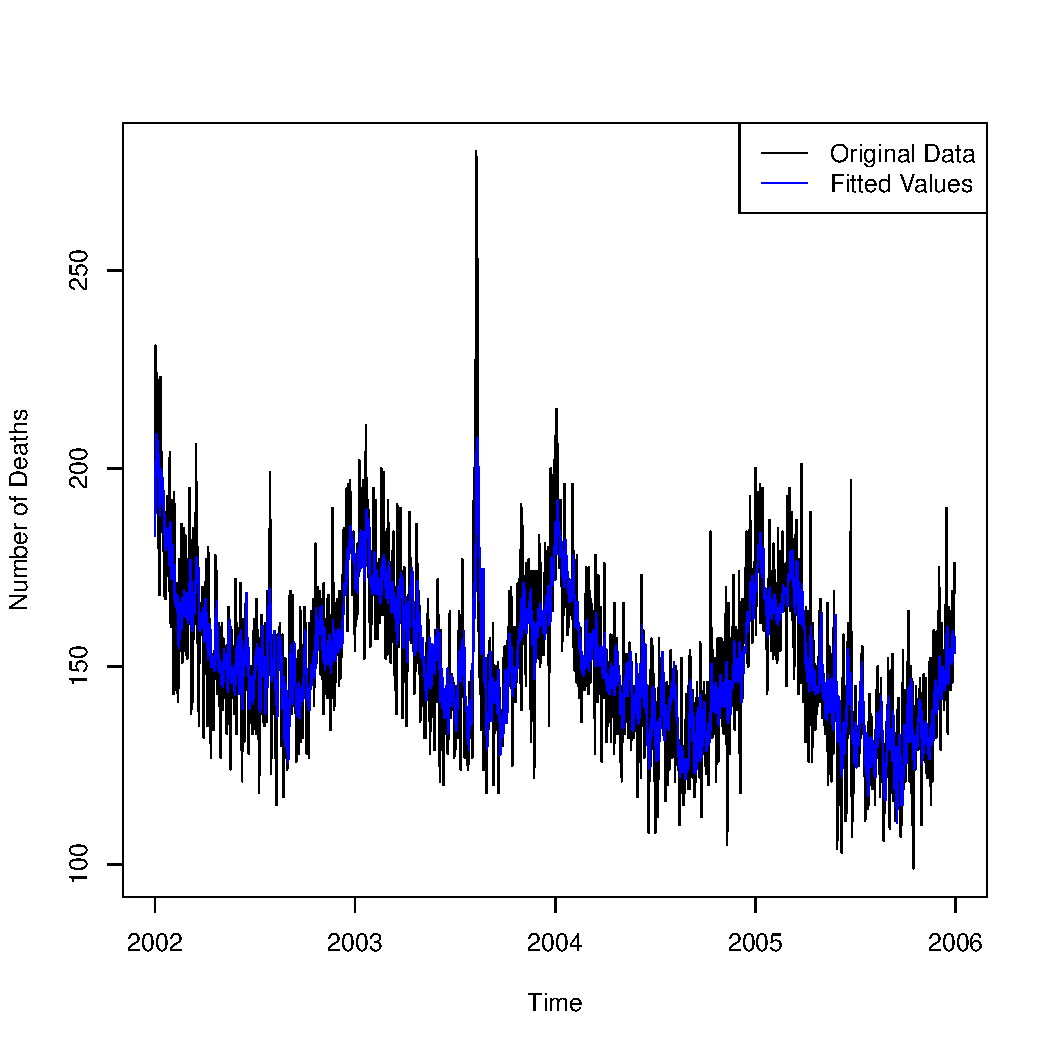
\includegraphics[width=0.50\textwidth]{figure/ts_3-1} }
\subfloat[Residuals over Time\label{fig:ts_32}]{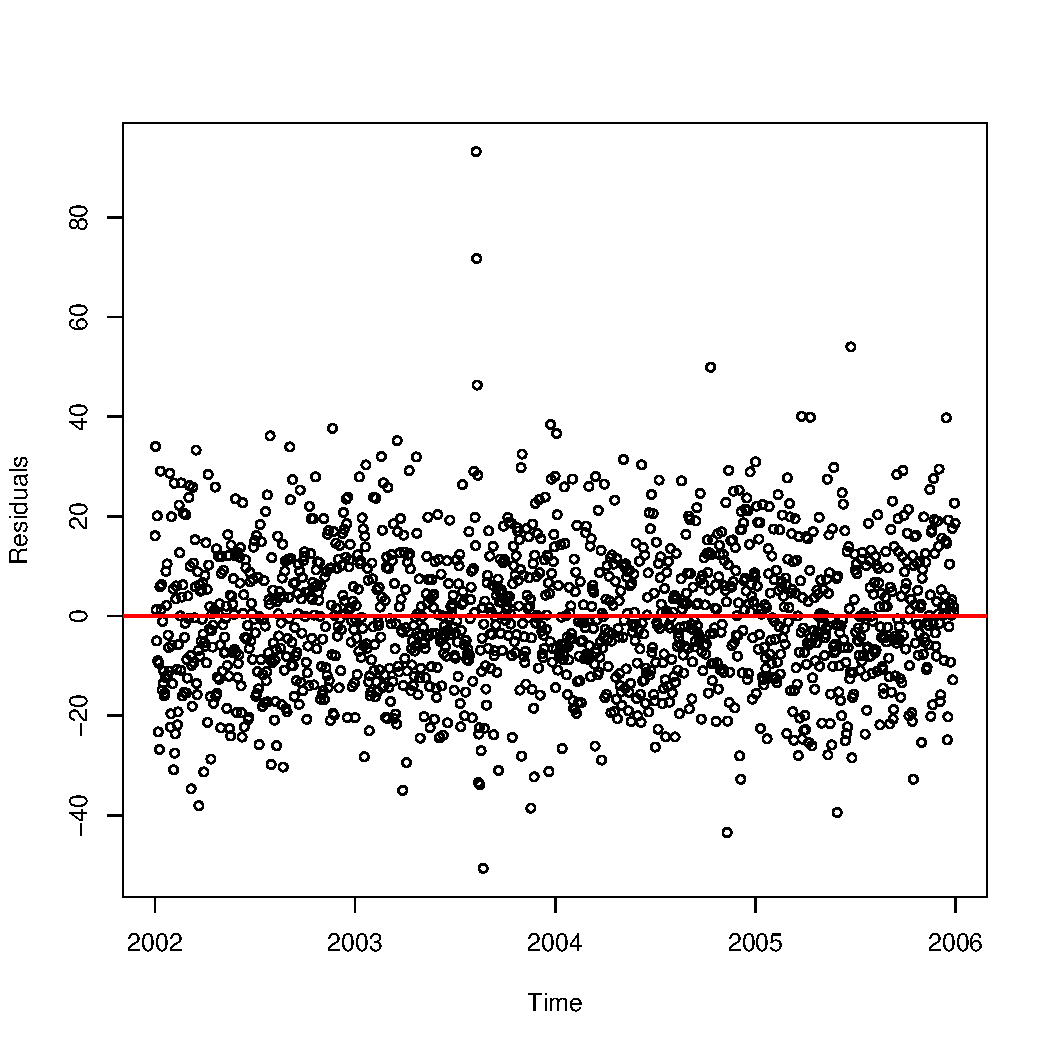
\includegraphics[width=0.50\textwidth]{figure/ts_3-2} }

}

\caption[Visualizing ARIMA Fit]{Visualizing ARIMA Fit}\label{fig:ts_3}
\end{figure}


\end{knitrout}

\begin{knitrout}
\definecolor{shadecolor}{rgb}{0.969, 0.969, 0.969}\color{fgcolor}\begin{figure}[H]

{\centering \subfloat[Fitted Values vs Original Series\label{fig:ts_41}]{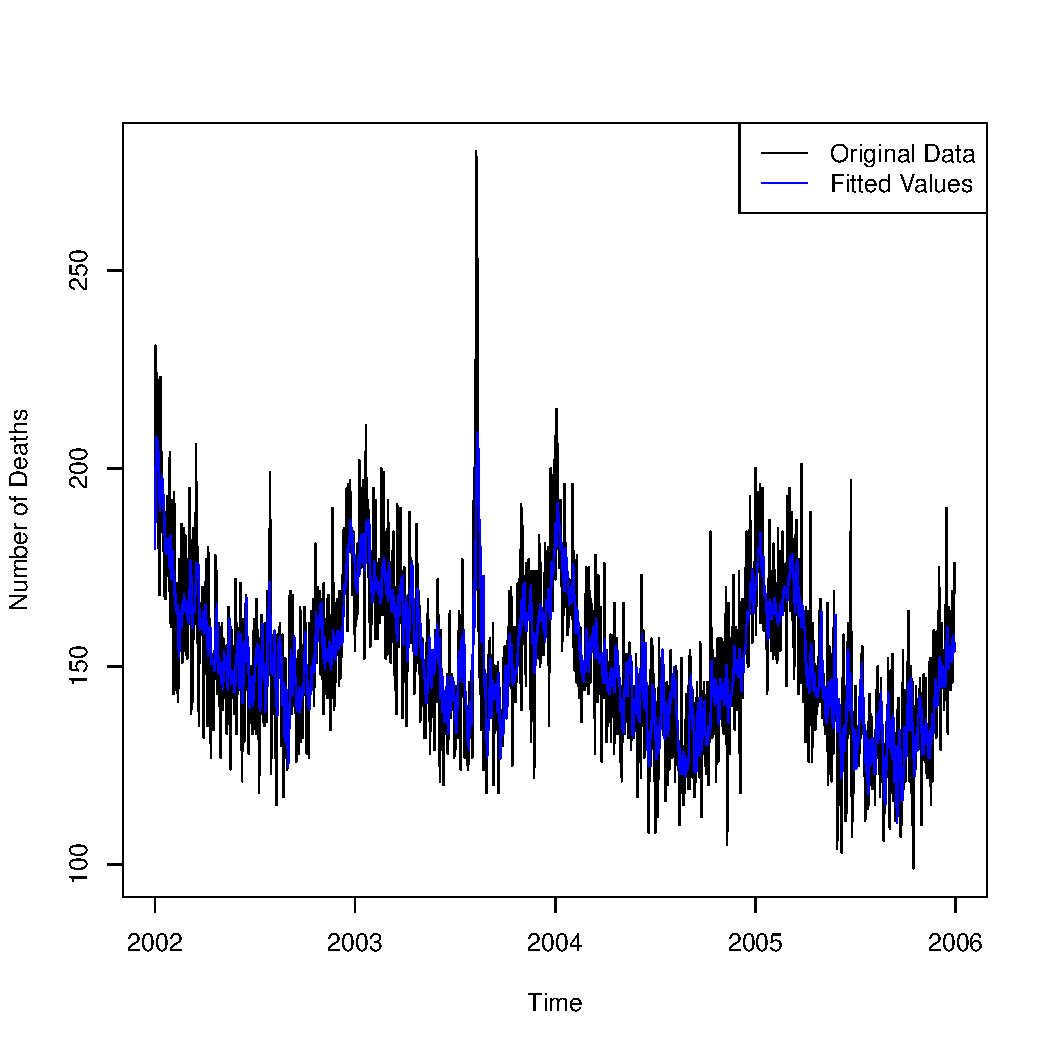
\includegraphics[width=0.50\textwidth]{figure/ts_4-1} }
\subfloat[Residuals over Time\label{fig:ts_42}]{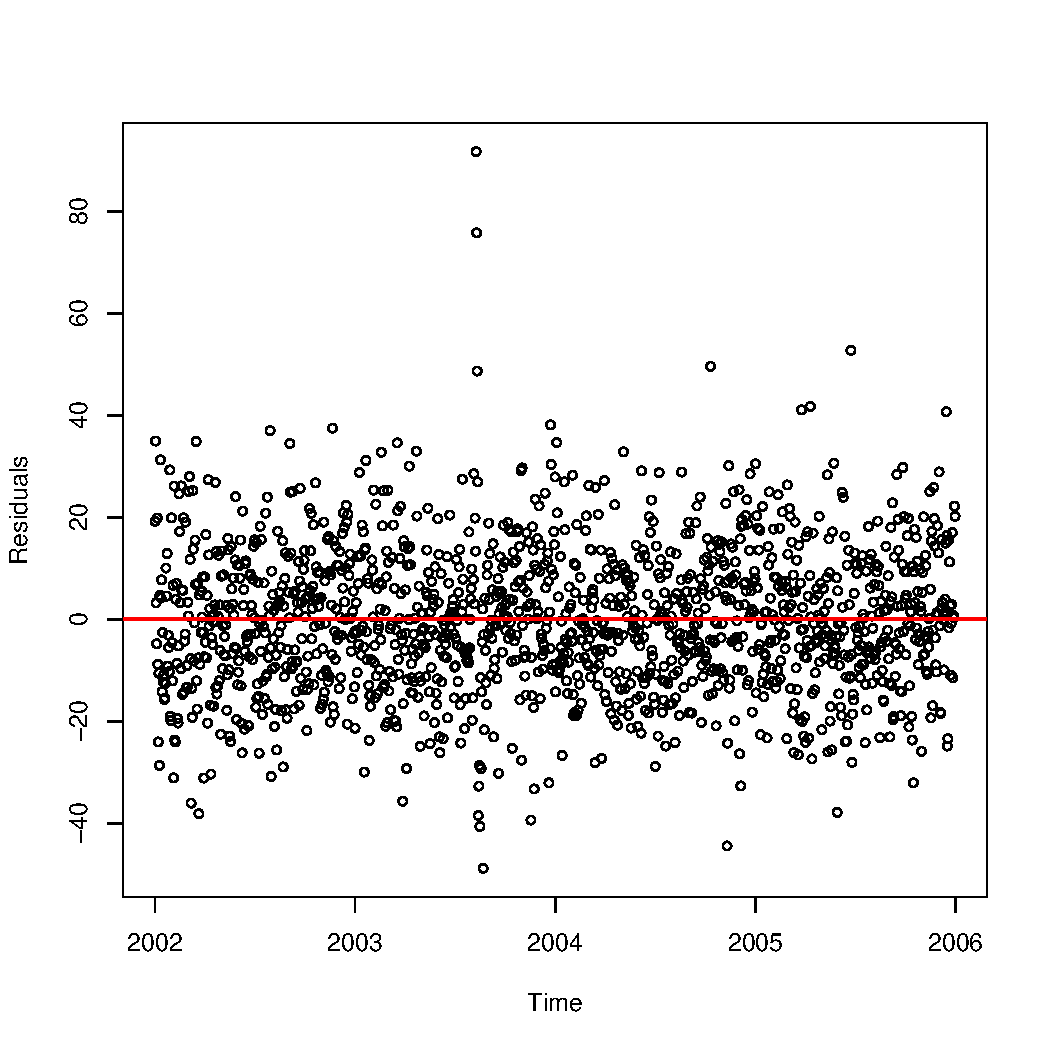
\includegraphics[width=0.50\textwidth]{figure/ts_4-2} }

}

\caption{Visualizing \texttt{auto.arima} Fit}\label{fig:ts_4}
\end{figure}


\end{knitrout}

The fitted values for both models fit the original data pretty well and they both capture the trend and seasonality of the data. Similarly, the residual plots for both models look good. The residual values are randomly distributed and centered around zero. Both plots show constant variance and have no apparent patterns. 

\subsubsection*{Model Validation}

\autoref{fig:ts_5} and \autoref{fig:ts_6} show the QQ plots and the ACF/PACF plots for the refitted time series regression models, corresponding to ARMA(1,1) and ARMA(2,8) respetively.

\begin{knitrout}
\definecolor{shadecolor}{rgb}{0.969, 0.969, 0.969}\color{fgcolor}\begin{figure}[H]

{\centering \subfloat[QQ Plot of Residuals\label{fig:ts_51}]{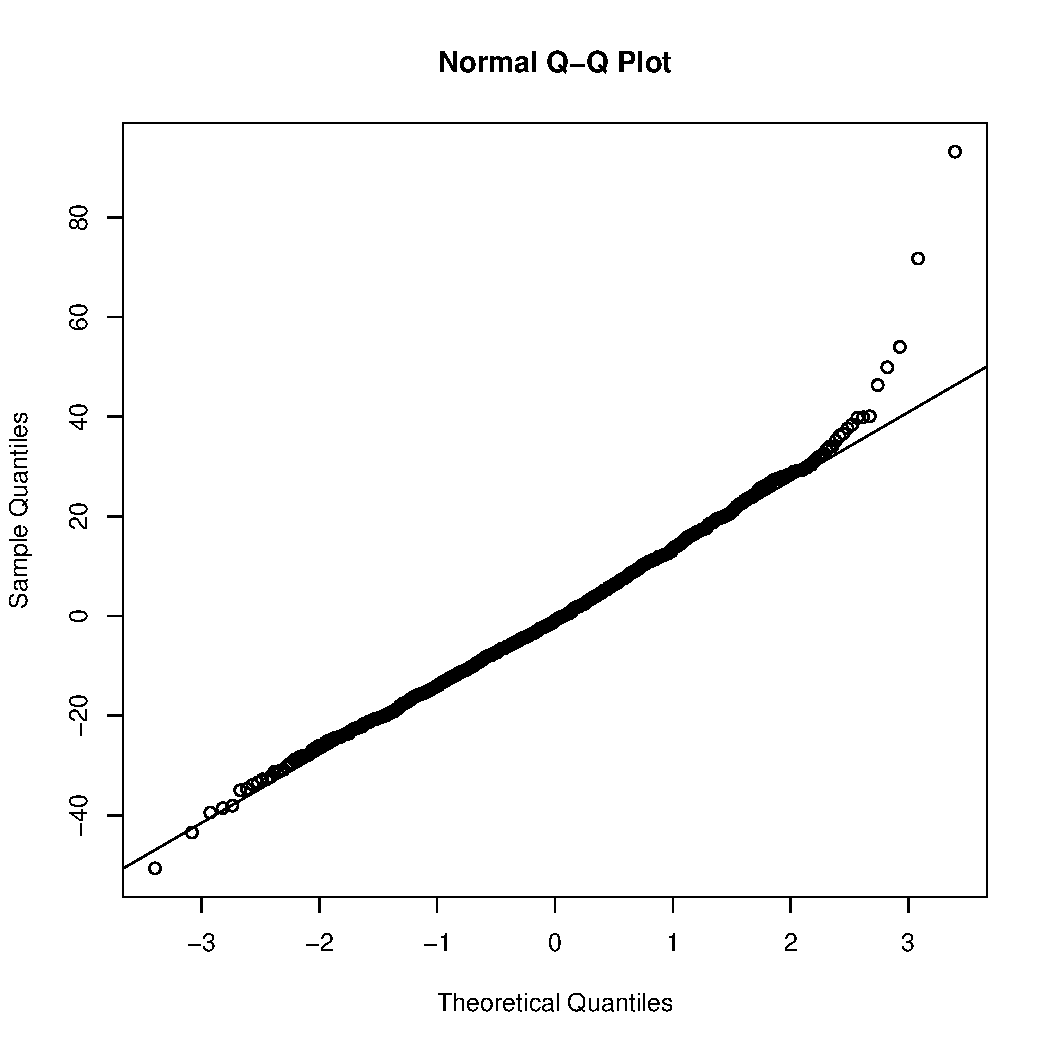
\includegraphics[width=0.50\textwidth]{figure/ts_5-1} }
\subfloat[ACF/PACF of Residuals\label{fig:ts_52}]{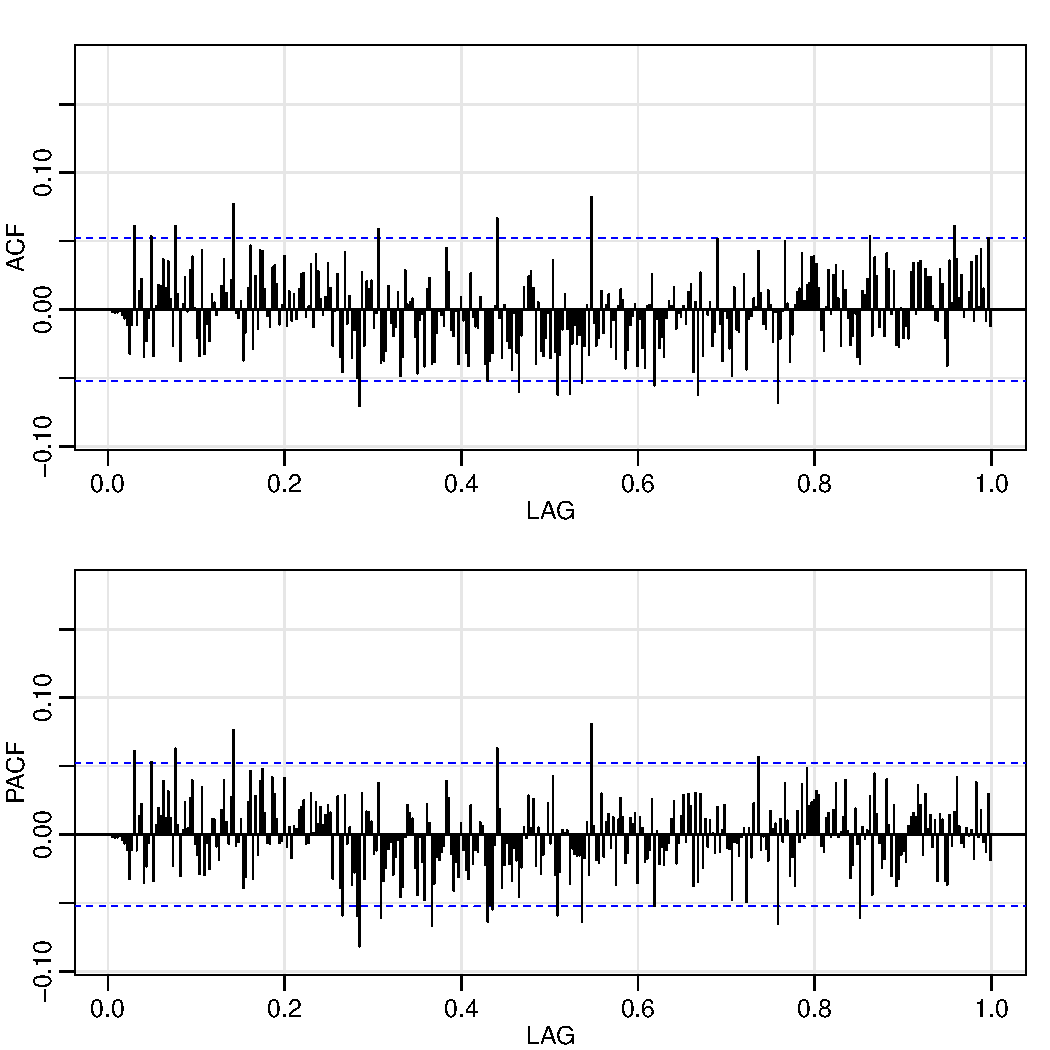
\includegraphics[width=0.50\textwidth]{figure/ts_5-2} }

}

\caption[Visualizing ARIMA Residuals]{Visualizing ARIMA Residuals}\label{fig:ts_5}
\end{figure}


\end{knitrout}

\begin{knitrout}
\definecolor{shadecolor}{rgb}{0.969, 0.969, 0.969}\color{fgcolor}\begin{figure}[H]

{\centering \subfloat[QQ Plot of Residuals\label{fig:ts_61}]{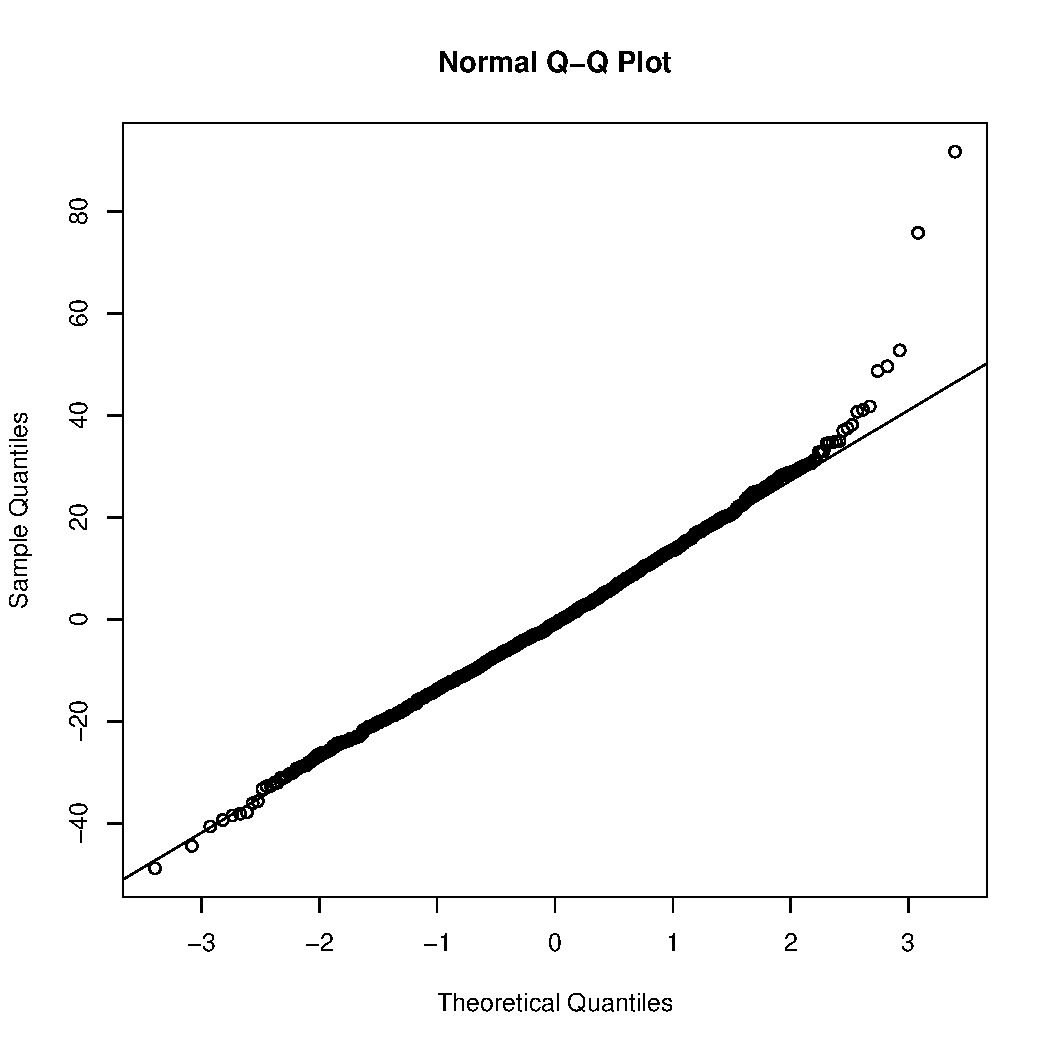
\includegraphics[width=0.50\textwidth]{figure/ts_6-1} }
\subfloat[ACF/PACF of Residuals\label{fig:ts_62}]{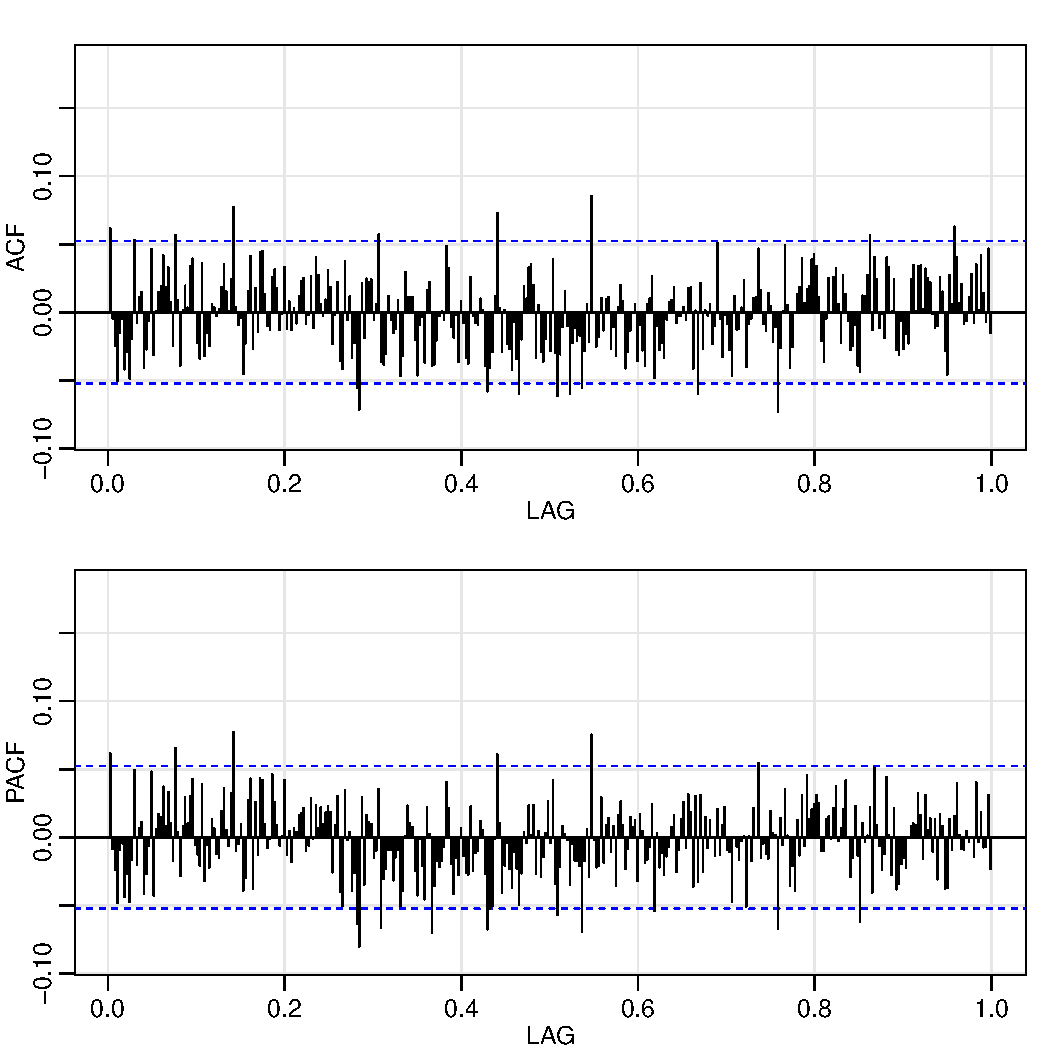
\includegraphics[width=0.50\textwidth]{figure/ts_6-2} }

}

\caption{Visualizing \texttt{auto.arima} Residuals}\label{fig:ts_6}
\end{figure}


\end{knitrout}

For both QQ plots, the points follow the normal QQ line, with the upper side having a slightly heavy tail. Unlike OLS, majority of the ACF and PACF values are within the confidence bands, meaning these values do not depend on lag. From all plots above, we can conclude that the new residuals for both ARMA(2,8) and ARMA(1,1) model are white noise. 

With all the evidence, we can say that both models do a equally good job in model fitting. However, here we will pick the results produced by \texttt{auto.arima} (residuals follow ARMA(1,1)) to proceed due to the simplicity of the model.

\subsubsection*{Model Forecasting}

\autoref{fig:ts_7} shows the forecast results for \texttt{auto.arima}. From the plot, we see that the point estimate do well only in the beginning of the prediction period. The model does capture the downward trend of the series, the daily volatility, and predicts some level of seasonality, but the predicted cycle is not in sync with the original series. The 95\% confidence interval are fairly wide, and share the same patterns as the point estimate. 

\begin{knitrout}
\definecolor{shadecolor}{rgb}{0.969, 0.969, 0.969}\color{fgcolor}\begin{figure}[H]

{\centering 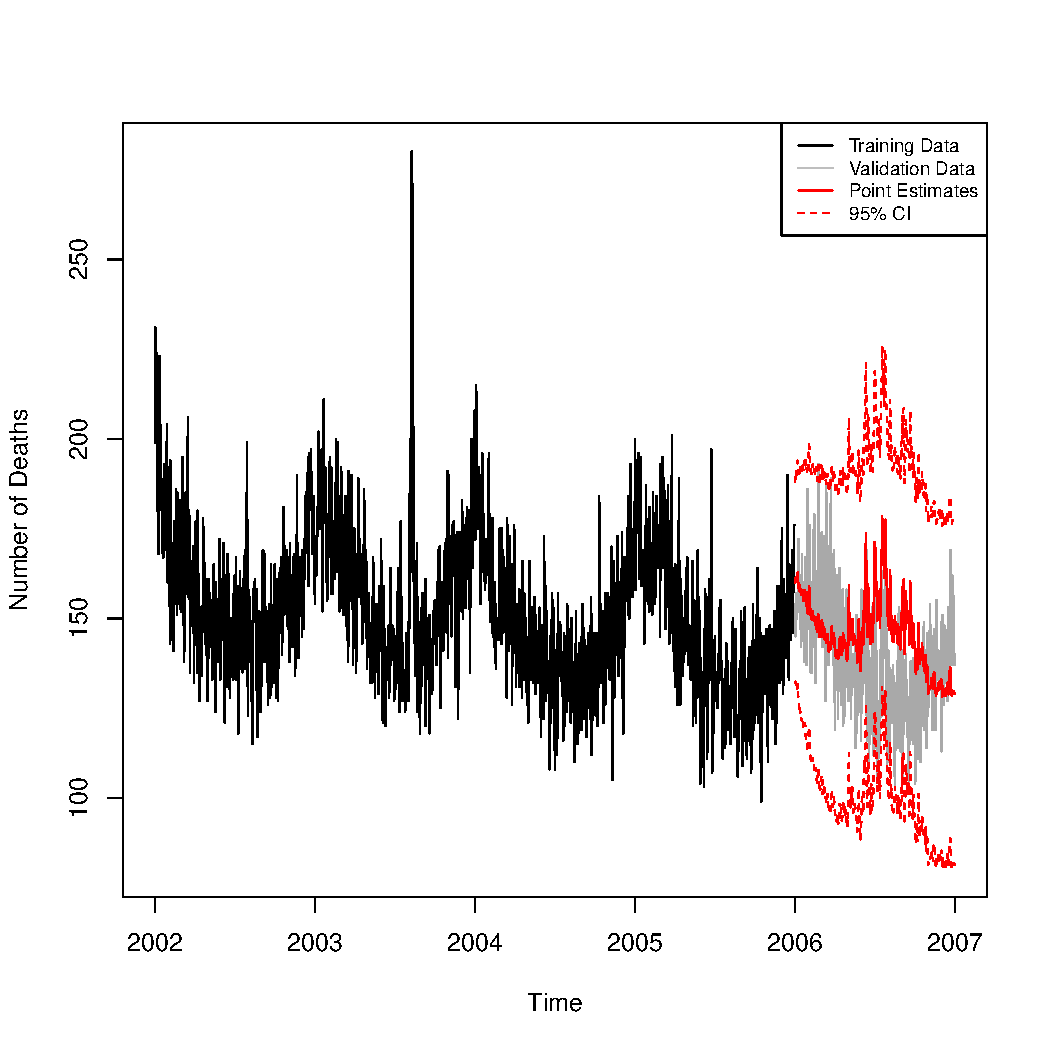
\includegraphics[width=0.65\textwidth]{figure/ts_7-1} 

}

\caption{Visualizing \texttt{auto.arima} Forecasts}\label{fig:ts_7}
\end{figure}


\end{knitrout}

\subsubsection*{Model Inference}

\autoref{tab:ts_reg} shows the coefficient and standard error for each variable in the time series regression. From the table, we see that \texttt{Adjusted Temperature} has high positive coefficient. This means that there is a positive correlation between temperature and number of deaths: holding all the other variables fixed, when the temperature gets higher, number of deaths also increases. Ozone levels have a negative correlation with number of deaths and relative humidity has a positive correlation, though the results for both variables are insignificant within 95\% confidence interval (because the interval includes zero). Other variables that have significant coefficients are \texttt{ar1}, \texttt{ma1} and \texttt{(Adjusted Temperature)$^2$}.

% latex table generated in R 3.4.3 by xtable 1.8-3 package
% Sun Apr 28 23:57:55 2019
\begin{table}[ht]
\centering
\scalebox{1}{
\begin{tabular}{rrr}
  \hline
 & Estimate & Std. Error \\ 
  \hline
ar 1 & 0.99 & 0.00 \\ 
  ma 1 & -0.78 & 0.02 \\ 
  intercept & 13289.39 & 10715.63 \\ 
  Trend & -6.56 & 5.35 \\ 
  Adjusted Temperature & 1.41 & 0.17 \\ 
  (Adjusted Temperature)$^2$ & 0.12 & 0.02 \\ 
  Ozone & -0.04 & 0.03 \\ 
  Relative Humidity & 0.06 & 0.04 \\ 
  Day of Week & 0.18 & 0.17 \\ 
  Day of Month & -0.01 & 0.05 \\ 
   \hline
\end{tabular}
}
\caption{Time Series Estimated Coefficients} 
\label{tab:ts_reg}
\end{table}


\subsection{Vector Autoregression} \label{ssec:VAR}
\subsubsection*{Model Fitting}
\vspace{-20 pt}

\begin{knitrout}
\definecolor{shadecolor}{rgb}{0.969, 0.969, 0.969}\color{fgcolor}\begin{figure}[H]

{\centering \subfloat[Fitted Values vs Original Series\label{fig:var_21}]{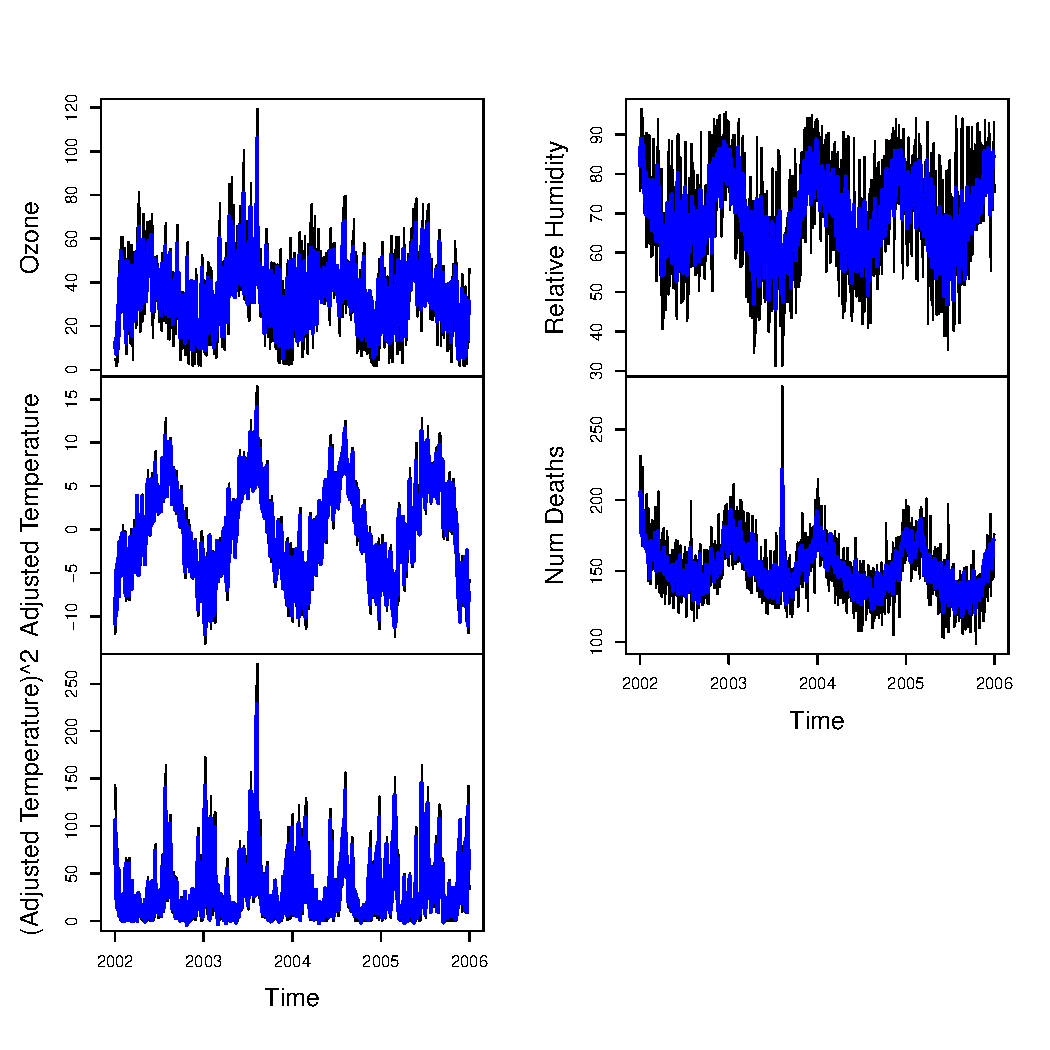
\includegraphics[width=0.45\textwidth]{figure/var_2-1} }
\subfloat[Residuals for Individual Series\label{fig:var_22}]{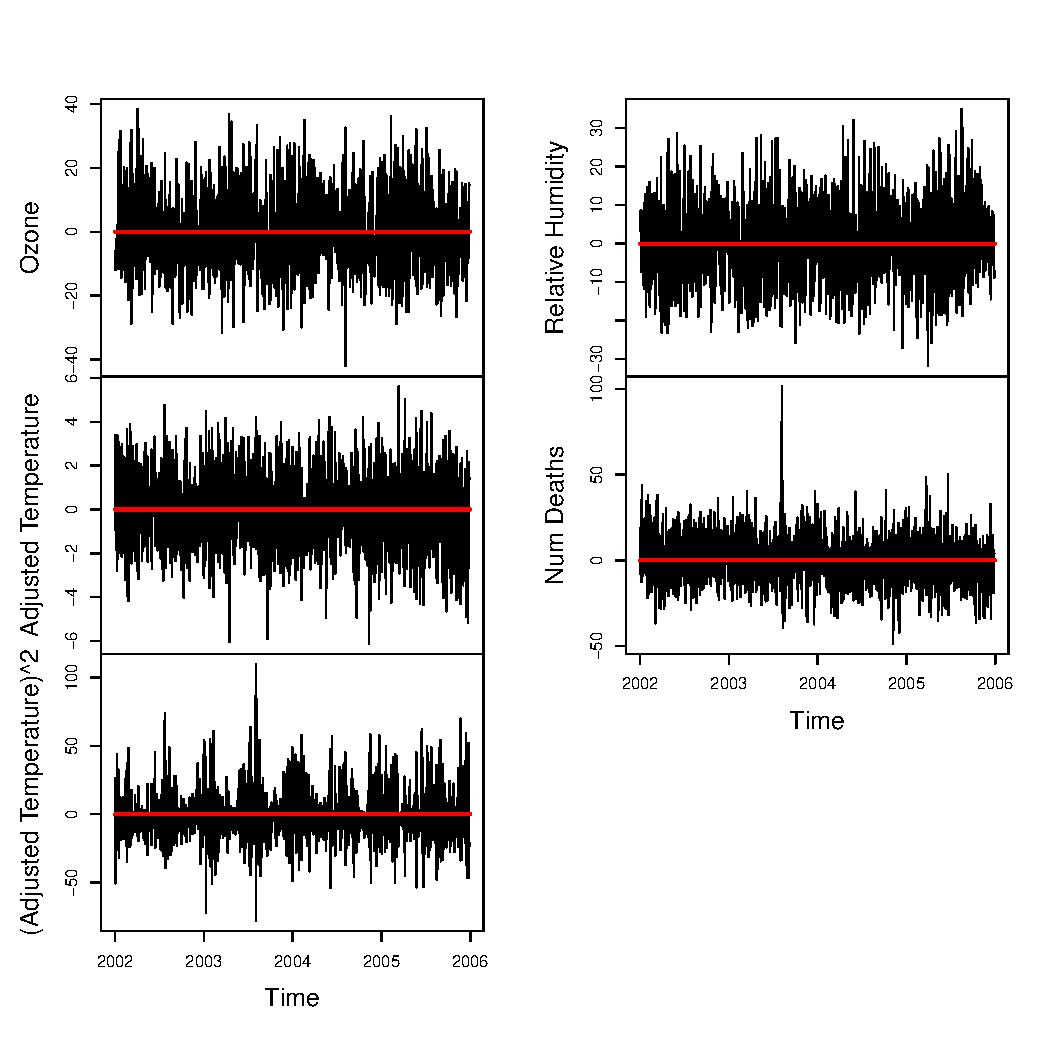
\includegraphics[width=0.45\textwidth]{figure/var_2-2} }

}

\caption[Visualizing VAR($p$=3, season=\texttt{NULL})]{Visualizing VAR($p$=3, season=\texttt{NULL})}\label{fig:var_2}
\end{figure}


\end{knitrout}

\vspace{-20 pt}

\begin{knitrout}
\definecolor{shadecolor}{rgb}{0.969, 0.969, 0.969}\color{fgcolor}\begin{figure}[H]

{\centering \subfloat[Fitted Values vs Original Series\label{fig:var_31}]{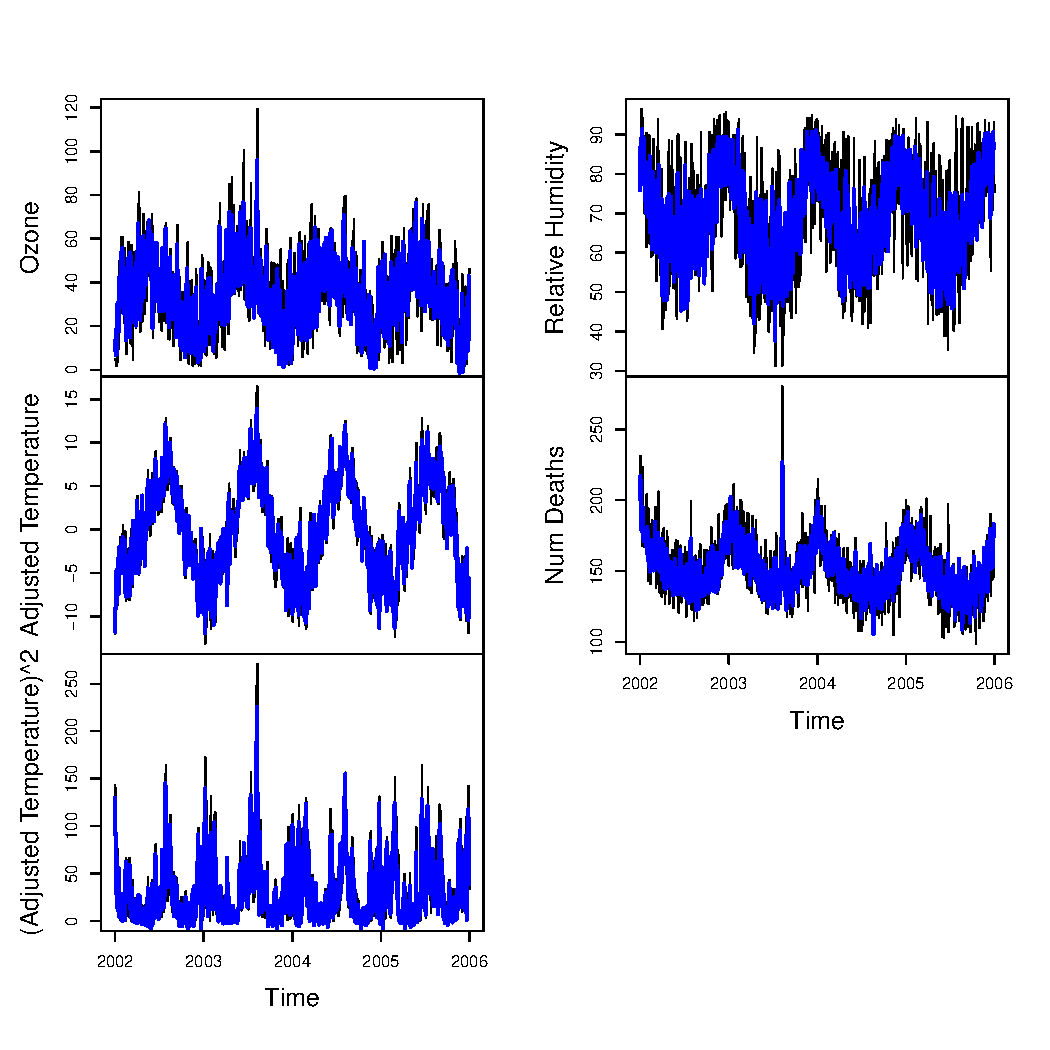
\includegraphics[width=0.45\textwidth]{figure/var_3-1} }
\subfloat[Residuals for Individual Series\label{fig:var_32}]{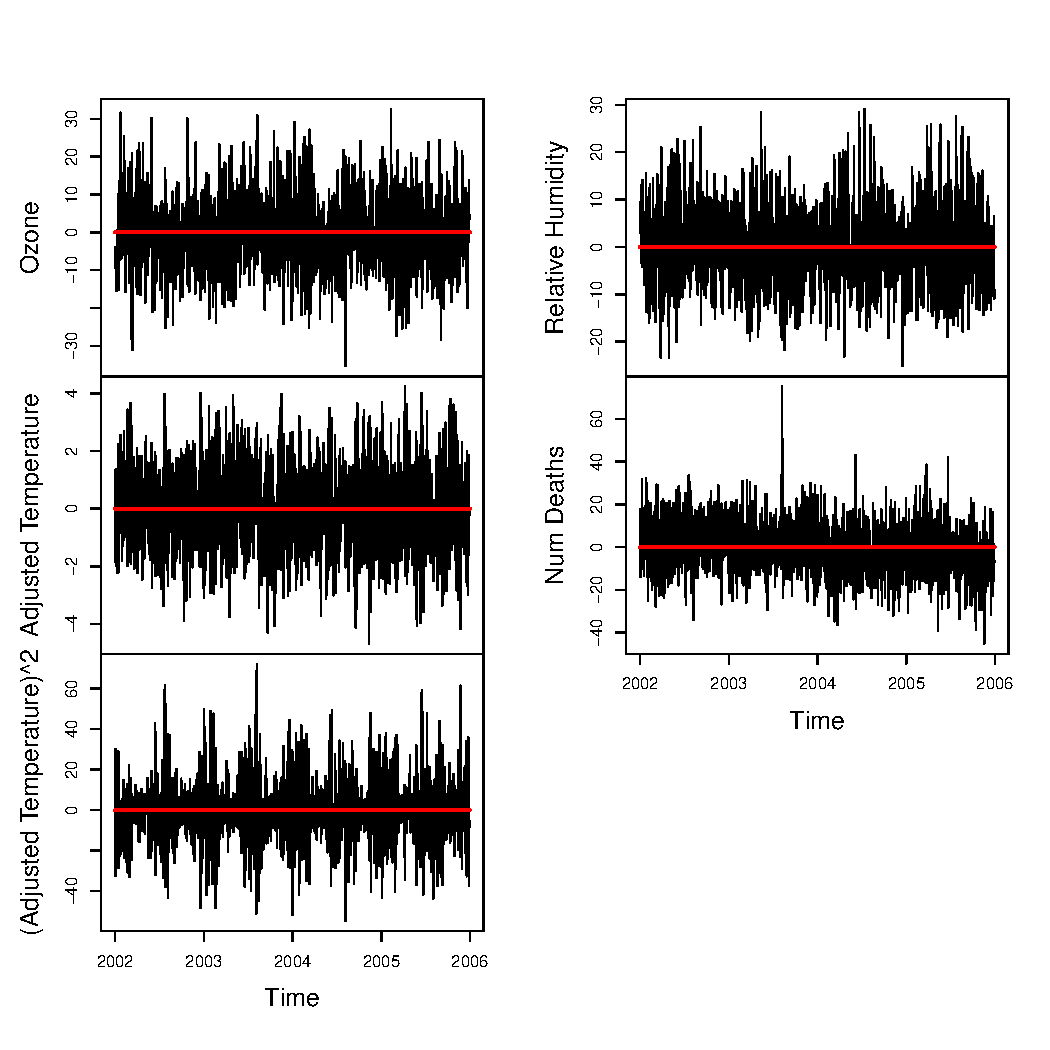
\includegraphics[width=0.45\textwidth]{figure/var_3-2} }

}

\caption[Visualizing VAR($p$=2, season=365)]{Visualizing VAR($p$=2, season=365)}\label{fig:var_3}
\end{figure}


\end{knitrout}

\autoref{fig:var_2} and~\autoref{fig:var_3} visualize the fitted values and the residuals for the VAR($p$=3, season=\texttt{NULL}) and VAR($p$=2, season=365) models. Between the two sets of figures the plots appear nearly identical with the second model slightly capturing the variability of the individual series more than the first model. This can be identified in the left hand plots where the fitted values in blue more closely follow the original data specifically in the \texttt{Ozone}, \texttt{Relative Humidity} and \texttt{Num Deaths} series for the second model. On the right hand side, the residuals are mostly centered around the line $y=0$ and maintain a constant variance over time except for the notable spike in 2003 and for the squared adjusted temperature series as a whole. 

\newpage
\begin{landscape}
\subsubsection*{Model Validation}
\vspace{-20 pt}

\begin{knitrout}
\definecolor{shadecolor}{rgb}{0.969, 0.969, 0.969}\color{fgcolor}\begin{figure}[H]

{\centering \subfloat[VAR($p$=3, season=\texttt{NULL})\label{fig:var_41}]{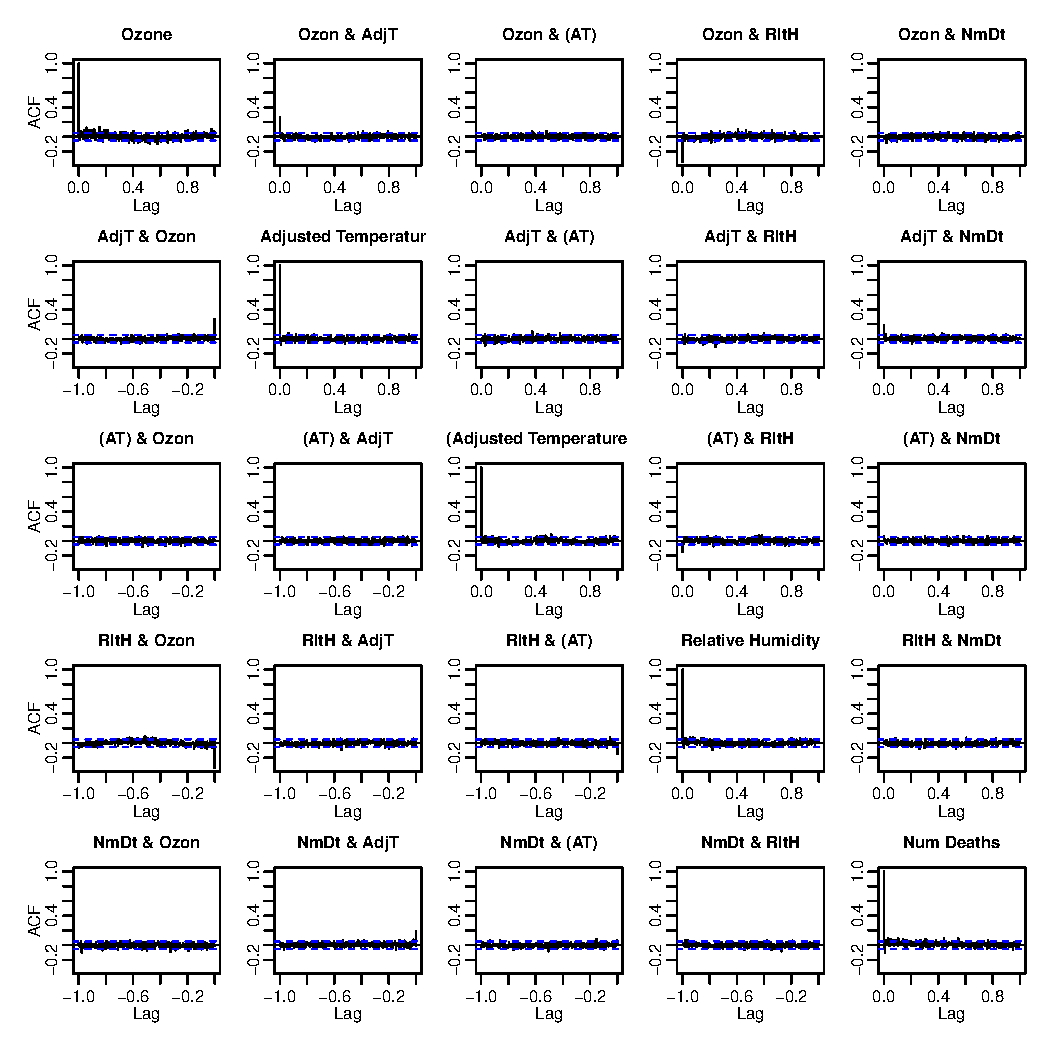
\includegraphics[width=0.65\textwidth]{figure/var_4-1} }
\subfloat[VAR($p$=2, season=365)\label{fig:var_42}]{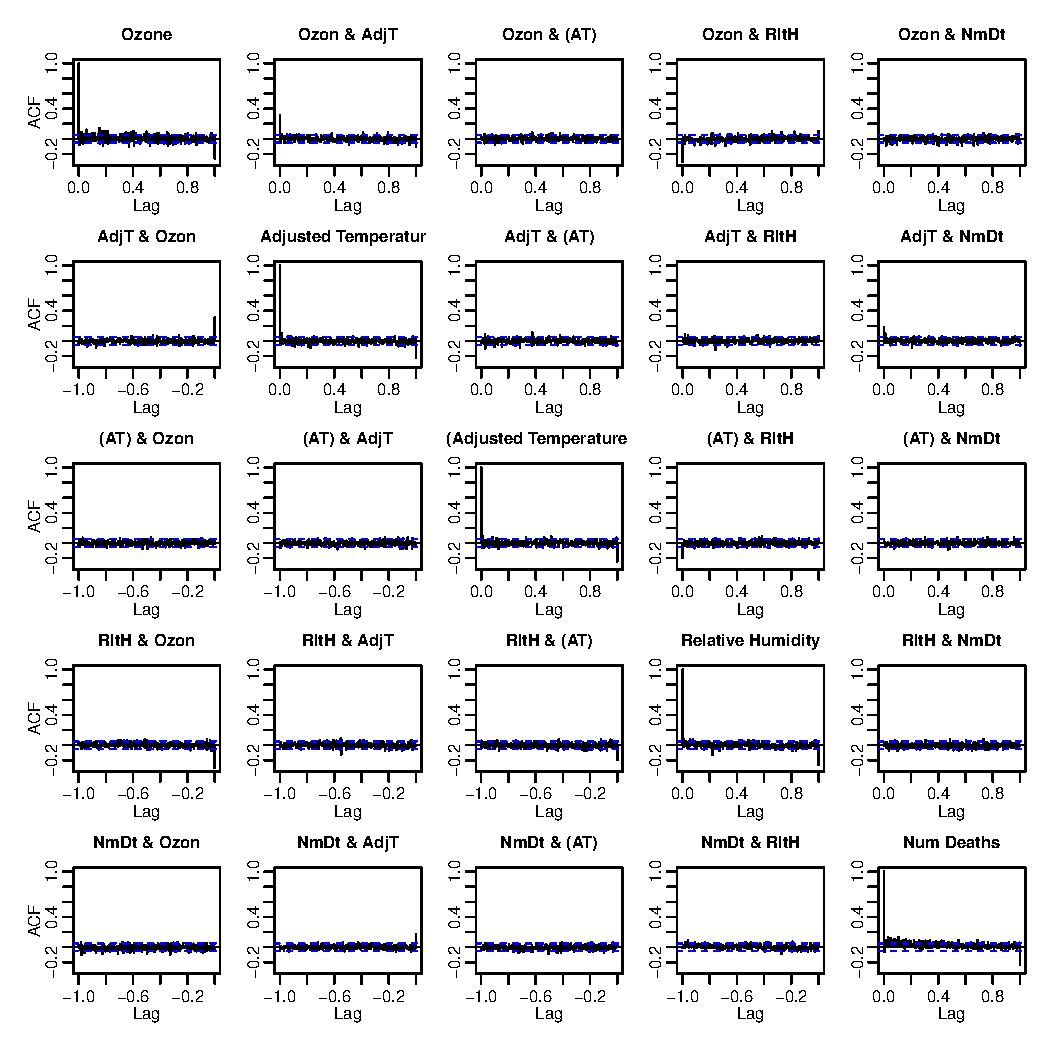
\includegraphics[width=0.65\textwidth]{figure/var_4-2} }

}

\caption[ACF/CCF Plots]{ACF/CCF Plots}\label{fig:var_4}
\end{figure}


\end{knitrout}

\autoref{fig:var_4} features the ACF/CCF plots for the VAR($p$=3, season=\texttt{NULL}) and VAR($p$=2, season=365) models. From this extensive grid of plots we can see that the residuals from the two models appear to come from a white noise process as indicated by the lack of statistically signficant non-zero auto/cross-correlations. It is also important to note that some of the ACF plots for the VAR($p$=2, season=365) model have a slight statistically significant value at lag 365 which suggests the data still needs some further manipulation.
\end{landscape}

\subsubsection*{Model Forecasting}
\vspace{-20 pt}

\begin{knitrout}
\definecolor{shadecolor}{rgb}{0.969, 0.969, 0.969}\color{fgcolor}\begin{figure}[H]

{\centering \subfloat[VAR($p$=3, season=\texttt{NULL})\label{fig:var_51}]{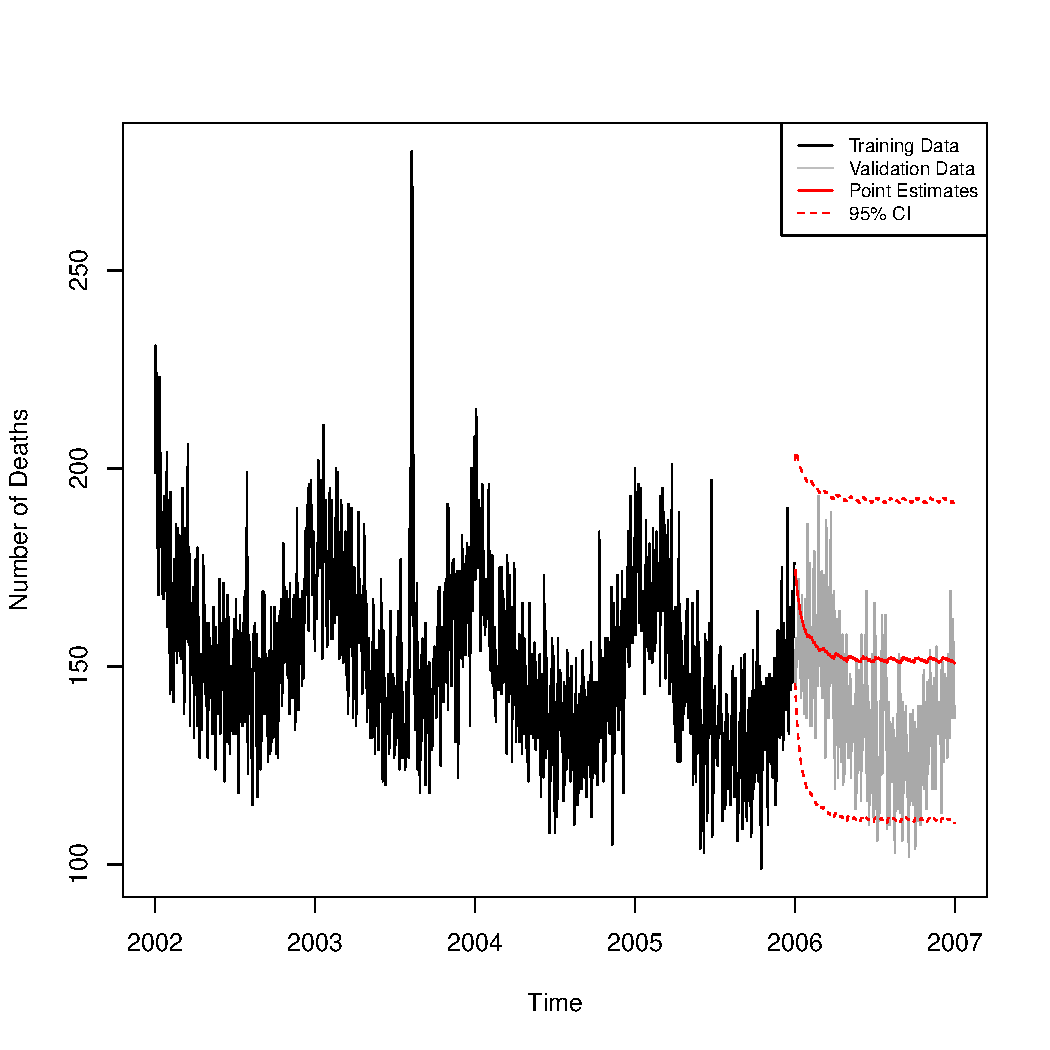
\includegraphics[width=0.50\textwidth]{figure/var_5-1} }
\subfloat[VAR($p$=2, season=365)\label{fig:var_52}]{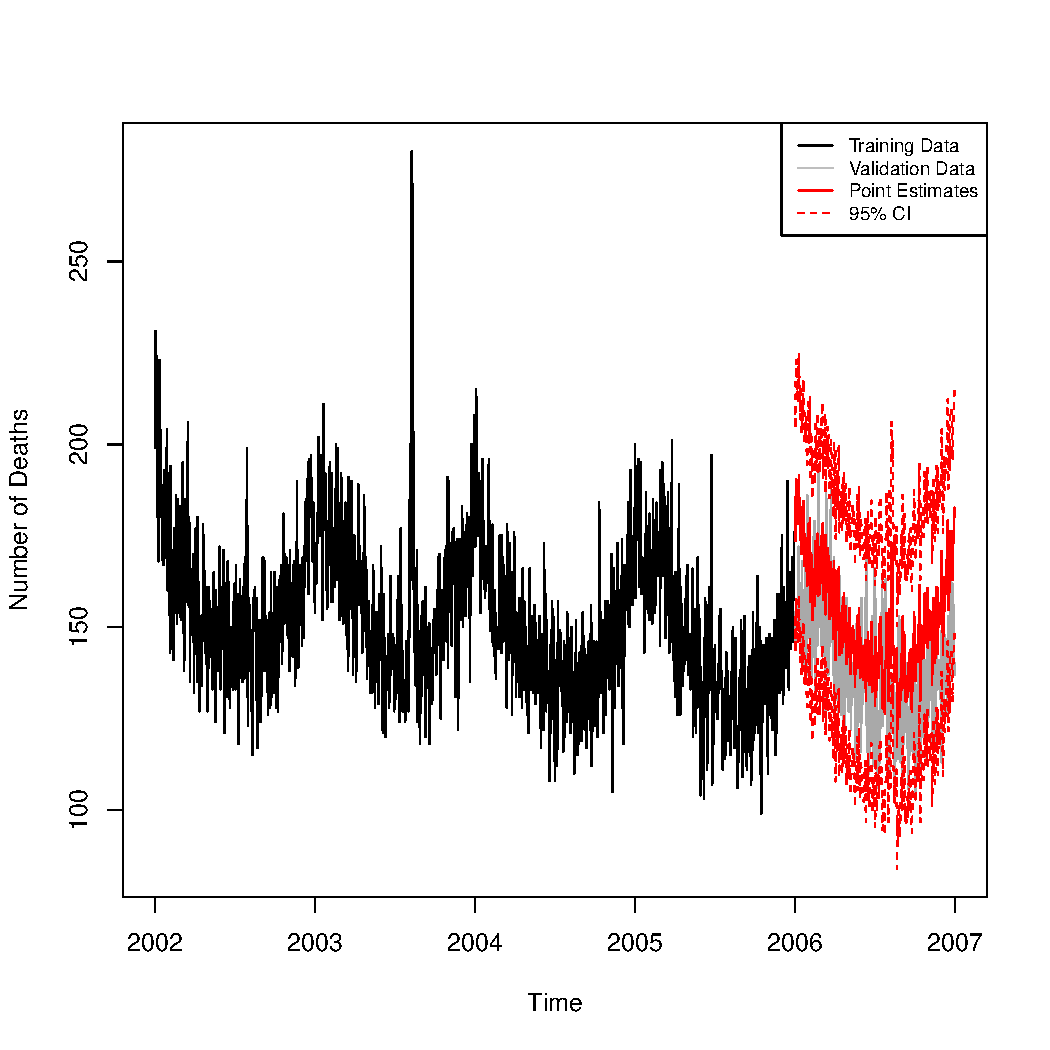
\includegraphics[width=0.50\textwidth]{figure/var_5-2} }

}

\caption[Visualizing Forecasting]{Visualizing Forecasting}\label{fig:var_5}
\end{figure}


\end{knitrout}

\autoref{fig:var_5} depicts the predictions for the testing data with the VAR($p$=3, season=\texttt{NULL}) and VAR($p$=2, season=365). \autoref{fig:var_5} (a) has an overall poor fit with the point estimates but the 95\% confidence interval mostly contains the value from the testing data. These predictions also capture the decreasing trend that the original series displays. \autoref{fig:var_5} (b) has a much better fit and the point estimates follow the observed testing data much very well as well as the 95\% confidence intervals capturing the test data within its bounds. Additionally, the point estimates and confidence intervals exhibit the same seasonal and daily volatility that the original data exhibits. This difference in quality of the fits can likely be attributed to the \texttt{seasonal} parameter. The inclusion of this parameter provides the second model with an additional 365 estimated coefficients. For this reason we will be examining the more parsimonious model, VAR($p$=3, season=\texttt{NULL}) since we are more interested in the inference capabilities of our model. It is worth noting how excellent the fit for the second model is and it should be kept in mind for further analysis. 

\subsubsection*{Model Inference}

% latex table generated in R 3.4.3 by xtable 1.8-3 package
% Sun Apr 28 23:58:11 2019
\begin{table}[ht]
\centering
\scalebox{0.75}{
\begin{tabular}{rrrrr}
  \hline
 & Estimate & Std. Error & t value & Pr($>|t|$) \\ 
  \hline
Ozone lag 1 & 0.043 & 0.035 & 1.229 & 2.19E-01 \\ 
  Adjusted Temperature lag 1 & 0.466 & 0.222 & 2.102 & 3.57E-02 \\ 
  (Adjusted Temperature)$^2$ lag 1 & 0.102 & 0.020 & 5.028 & 5.58E-07 \\ 
  Relative Humidity lag 1 & 0.016 & 0.039 & 0.402 & 6.88E-01 \\ 
  Num Deaths lag 1 & 0.280 & 0.026 & 10.600 & 2.48E-25 \\ 
  Ozone lag 2 & 0.074 & 0.043 & 1.726 & 8.46E-02 \\ 
  Adjusted Temperature lag 2 & -0.737 & 0.306 & -2.408 & 1.62E-02 \\ 
  (Adjusted Temperature)$^2$ lag 2 & -0.009 & 0.027 & -0.343 & 7.32E-01 \\ 
  Relative Humidity lag 2 & 0.035 & 0.042 & 0.829 & 4.07E-01 \\ 
  Num Deaths lag 2 & 0.185 & 0.027 & 6.858 & 1.03E-11 \\ 
  Ozone lag 3 & -0.055 & 0.035 & -1.559 & 1.19E-01 \\ 
  Adjusted Temperature lag 3 & -0.636 & 0.225 & -2.823 & 4.82E-03 \\ 
  (Adjusted Temperature)$^2$ lag 3 & -0.023 & 0.020 & -1.148 & 2.51E-01 \\ 
  Relative Humidity lag 3 & -0.053 & 0.040 & -1.332 & 1.83E-01 \\ 
  Num Deaths lag 3 & 0.169 & 0.026 & 6.601 & 5.74E-11 \\ 
  Trend & 0.026 & 0.003 & 10.256 & 7.19E-24 \\ 
  Day of Week & 0.028 & 0.192 & 0.144 & 8.86E-01 \\ 
  Day of Month & -0.023 & 0.043 & -0.537 & 5.92E-01 \\ 
   \hline
\end{tabular}
}
\caption{\texttt{Num Deaths} Coefficients from VAR(3)} 
\label{tab:var_coef}
\end{table}


\autoref{tab:var_coef} displays the summary of the estimated coefficients of the VAR($p$=3, season=\texttt{NULL}) model when regressing onto \texttt{Num Deaths} at time $t$. Few of the estimated coefficients are statistically significant (using the unadjusted p-values) and even fewer have estimated coefficients that are not near 0. The most important coefficients to note here (given the current variables in the model) are the lagged coefficients for \texttt{Adjusted Temperature} and the lagged coefficients for \texttt{Num Deaths}. These coefficient estimates are fairly large which suggest that they have some relationship with \texttt{Num Deaths} in the current time period. Based on the signage of these coefficients an increase in \texttt{Adjusted Temperature} at $(t - 1)$ has an increased number of deaths at time $t$ and an increase in \texttt{Adjusted Temperature} at $(t-2)$ and $(t-3)$ have a decrease number of deaths at time $t$. Similarily, an increase in \texttt{Num Deaths} at all lags $1, 2, 3$ leads to an increase in the number of deaths at time $t$.

\subsection{Neural Network Autoregression} \label{ssec:NNAR}
\subsubsection*{Model Fitting}
\vspace{-20 pt}
\begin{knitrout}
\definecolor{shadecolor}{rgb}{0.969, 0.969, 0.969}\color{fgcolor}\begin{figure}[H]

{\centering \subfloat[Fitted Values vs Original Series\label{fig:nn_11}]{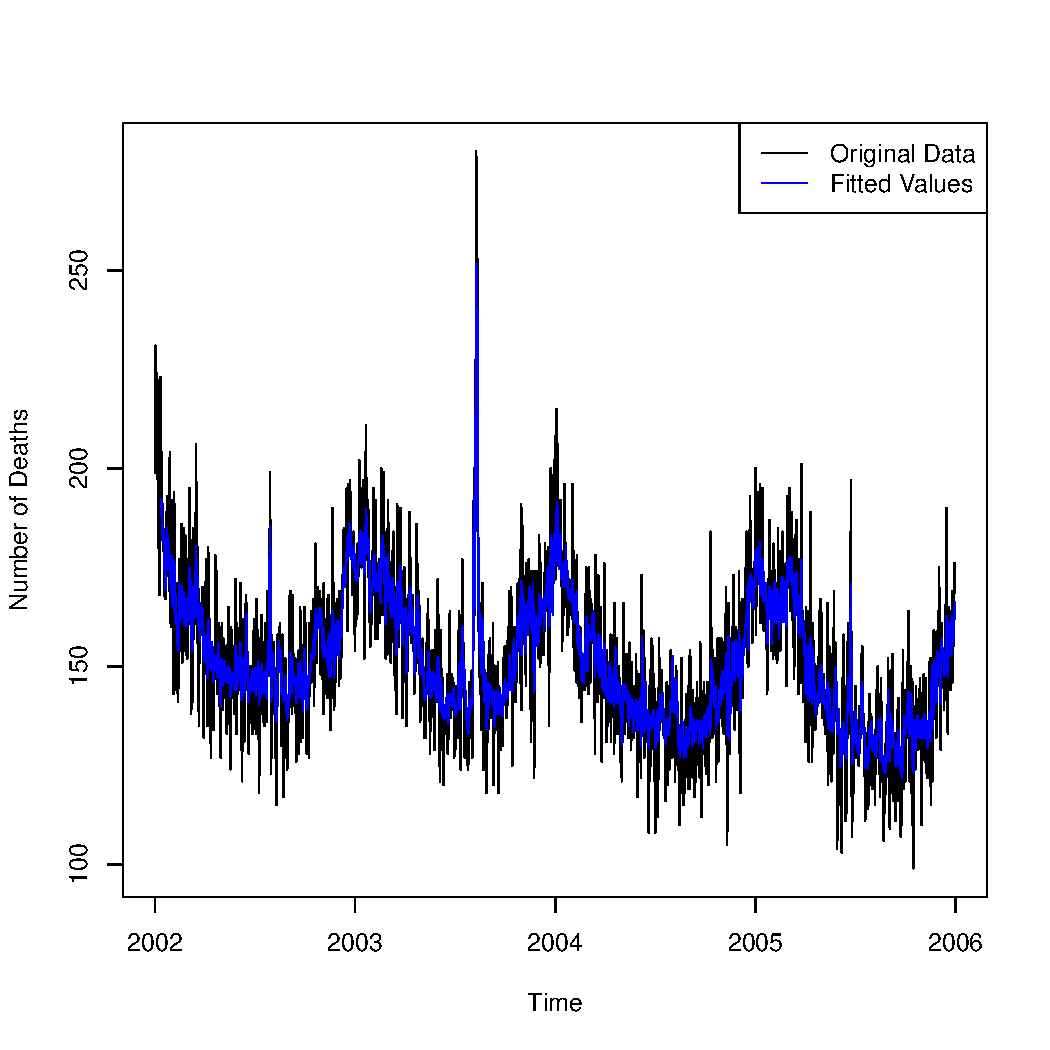
\includegraphics[width=0.50\textwidth]{figure/nn_1-1} }
\subfloat[Residuals over Time\label{fig:nn_12}]{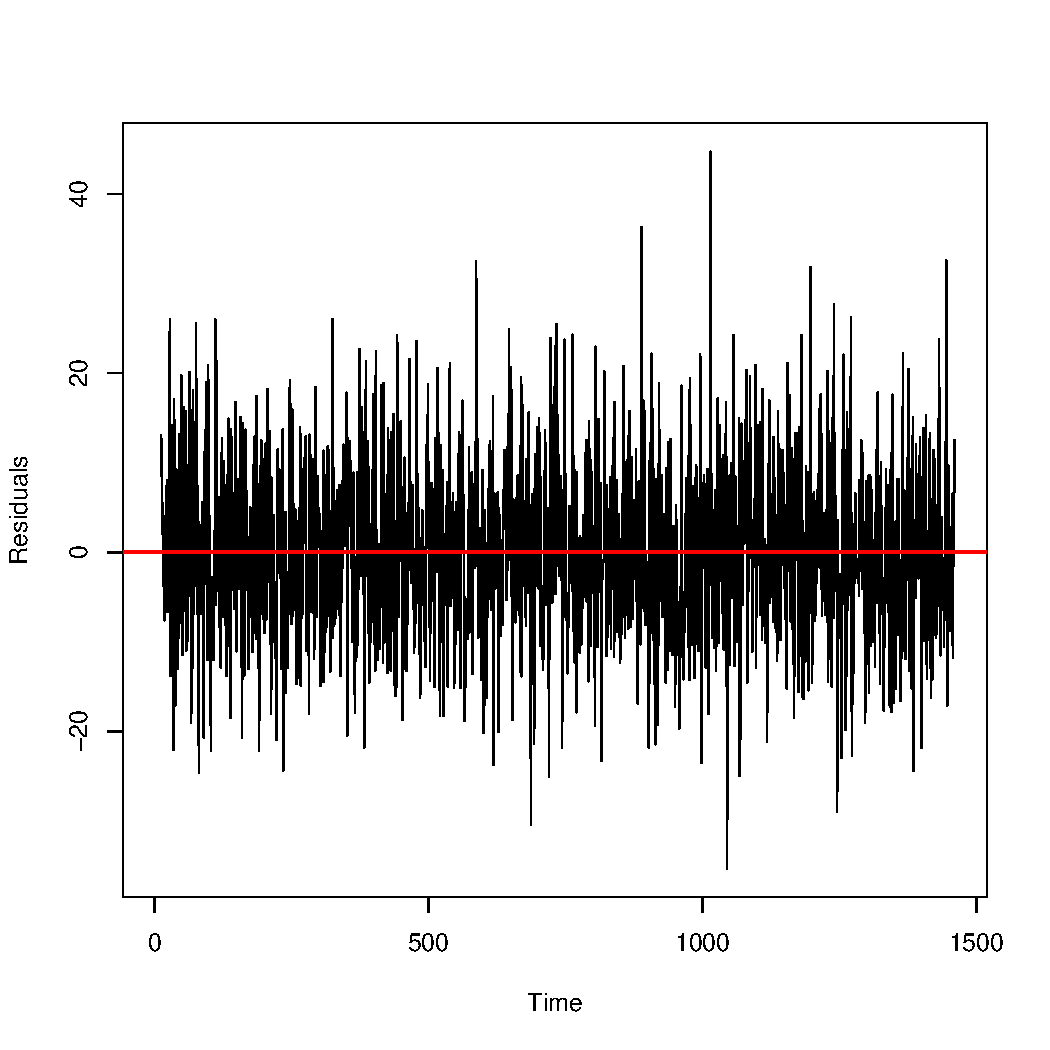
\includegraphics[width=0.50\textwidth]{figure/nn_1-2} }

}

\caption[Visualizing NNAR Fit]{Visualizing NNAR Fit}\label{fig:nn_1}
\end{figure}


\end{knitrout}

\autoref{fig:nn_1} illustrates the fitted values and residuals for the NNAR model described earlier. The model resulting from \texttt{nnetar()} is NNAR(10, 11).~\autoref{fig:nn_1} (a) shows that the fitted values nearly follow the original training data quite well.~\autoref{fig:nn_1} (b) shows that the residuals are almost evenly centered around $y=0$ and maintain a constant variance throughout time. Thus, this model is likely a good fit to the training dataset. 

\subsubsection*{Model Validation}
\vspace{-20 pt}
\begin{knitrout}
\definecolor{shadecolor}{rgb}{0.969, 0.969, 0.969}\color{fgcolor}\begin{figure}[H]

{\centering \subfloat[QQ Plot of Residuals\label{fig:nn_21}]{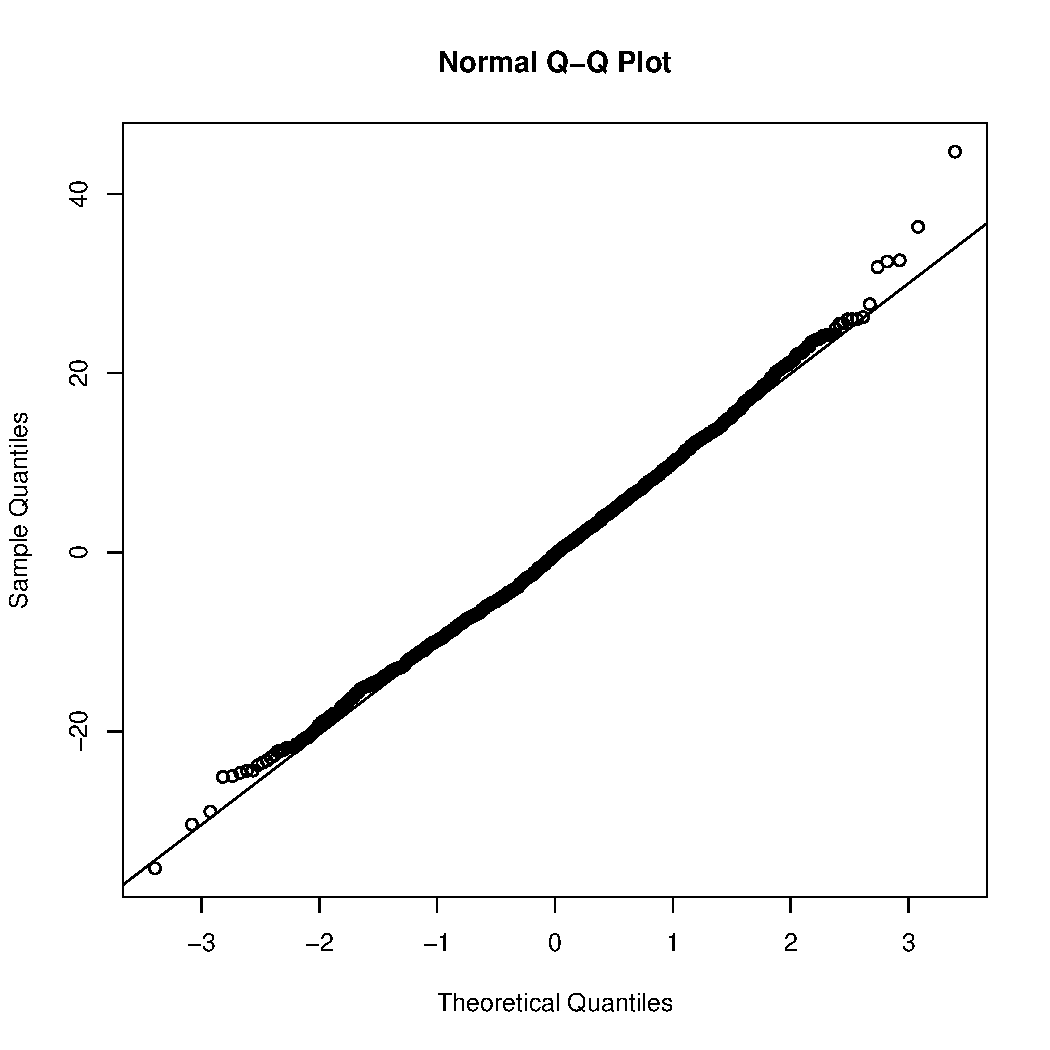
\includegraphics[width=0.50\textwidth]{figure/nn_2-1} }
\subfloat[ACF/PACF of Residuals\label{fig:nn_22}]{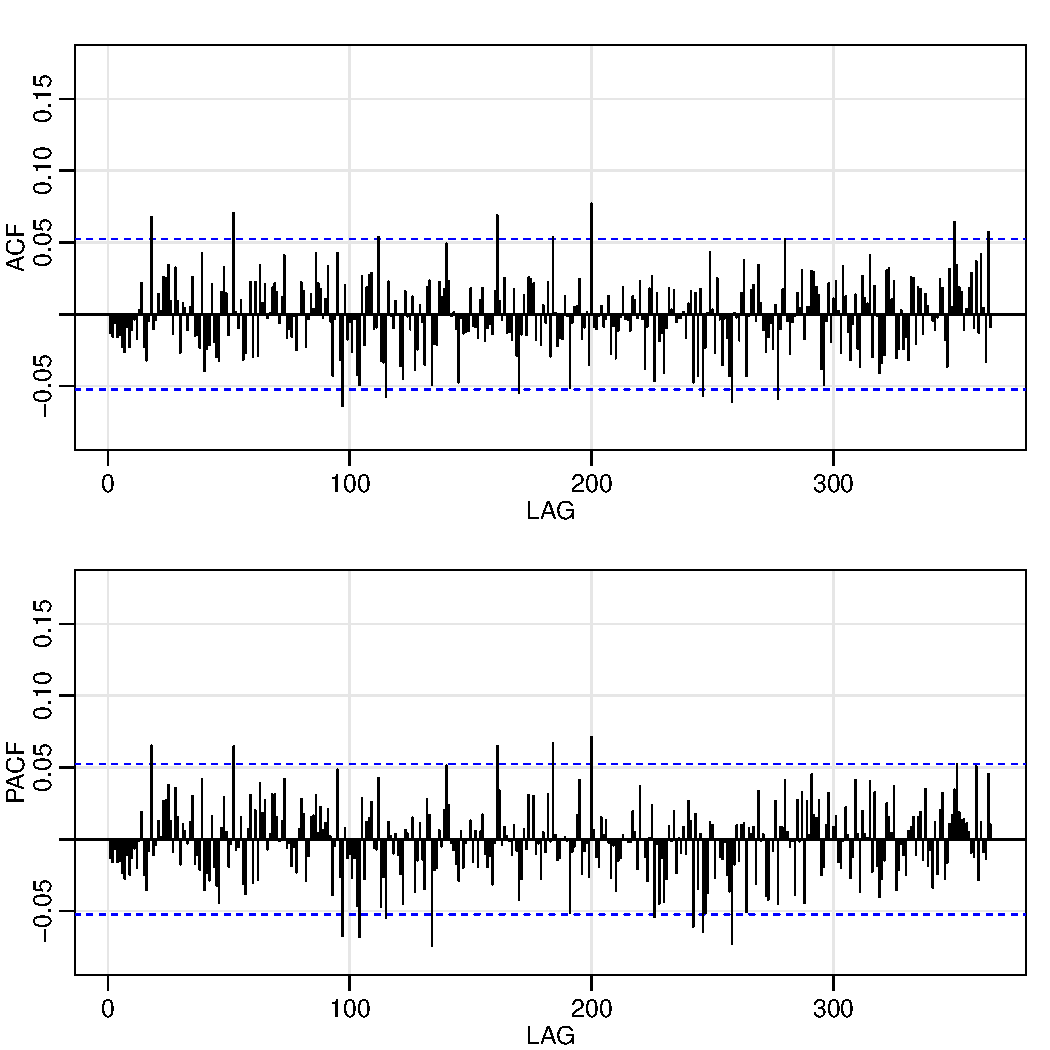
\includegraphics[width=0.50\textwidth]{figure/nn_2-2} }

}

\caption[Visualizing NNAR Residuals]{Visualizing NNAR Residuals}\label{fig:nn_2}
\end{figure}


\end{knitrout}

\autoref{fig:nn_2} displays the NNAR model residuals in more detail.~\autoref{fig:nn_2} (a) shows that the residuals approximately follow a normal distribution based on the QQ plot with only a slight deviation in the left tail.~\autoref{fig:nn_2} (b) shows the ACF/PACF plot which illustrate that the remaining residuals approximately follow a white noise distribution. Thus, supporting that this model does well in the training aspect.

\subsubsection*{Model Prediction}
\noindent\underline{\textbf{Forecasting Ahead}:}
\vspace{-20 pt}
\begin{knitrout}
\definecolor{shadecolor}{rgb}{0.969, 0.969, 0.969}\color{fgcolor}\begin{figure}[H]

{\centering 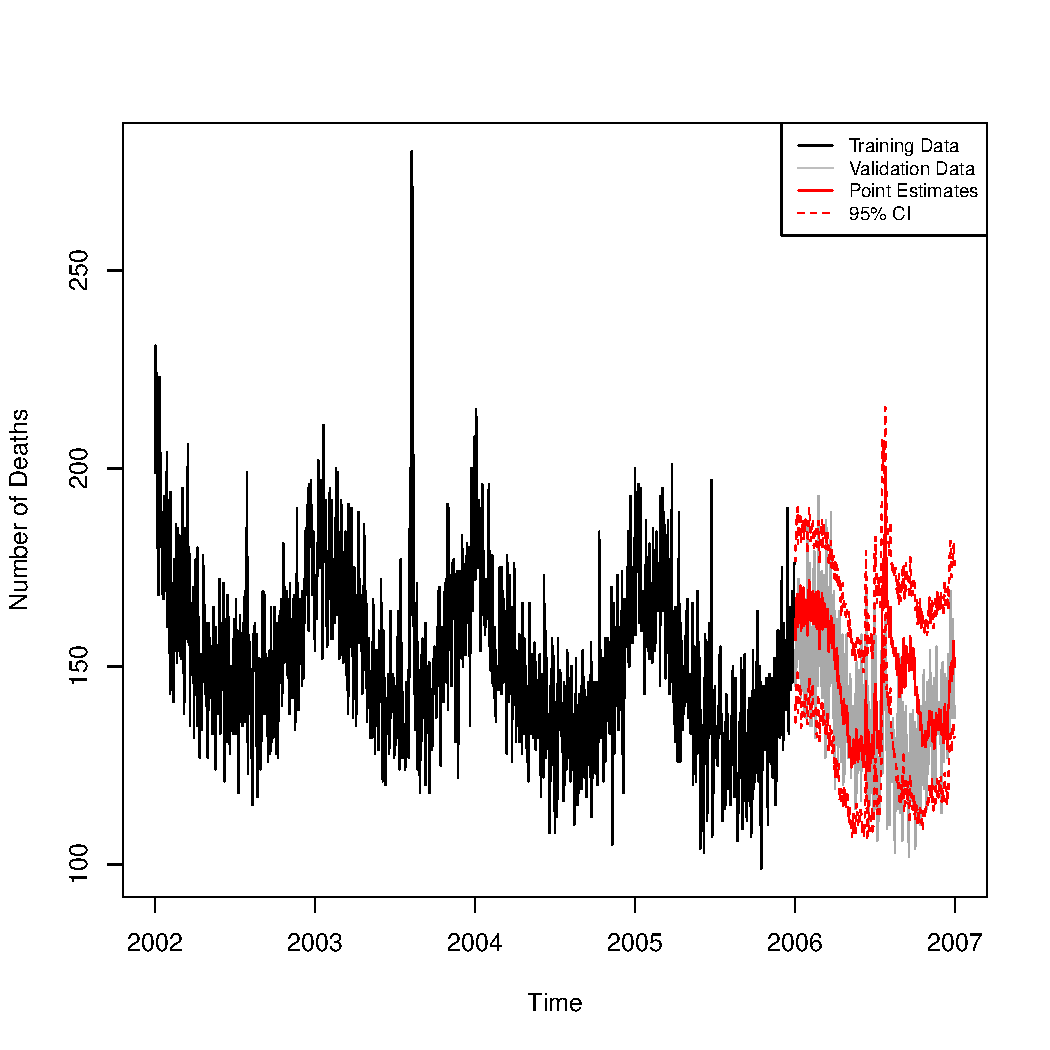
\includegraphics[width=0.65\textwidth]{figure/nn_3-1} 

}

\caption[Visualizing \texttt{NNAR} Forecasts]{Visualizing \texttt{NNAR} Forecasts}\label{fig:nn_3}
\end{figure}


\end{knitrout}

\autoref{fig:nn_3} displays the predictions for the testing data using the NNAR model. The point estimates do fairly well with prediction except for a period of time roughly half way through the testing year. The 95\% confidence interval also manages to capture most of the data within its bounds, with the exception of the same period of time as the point estimations. It is also important to note that the model manages to capture the overall seasonal trend and daily volatility that the original data displays. Thus, the generalizability of the model appear adequate but not great.

\noindent\underline{\textbf{Simulated Data}:}
\vspace{-20 pt}
\begin{knitrout}
\definecolor{shadecolor}{rgb}{0.969, 0.969, 0.969}\color{fgcolor}\begin{figure}[H]

{\centering \subfloat[Original Series\label{fig:nn_41}]{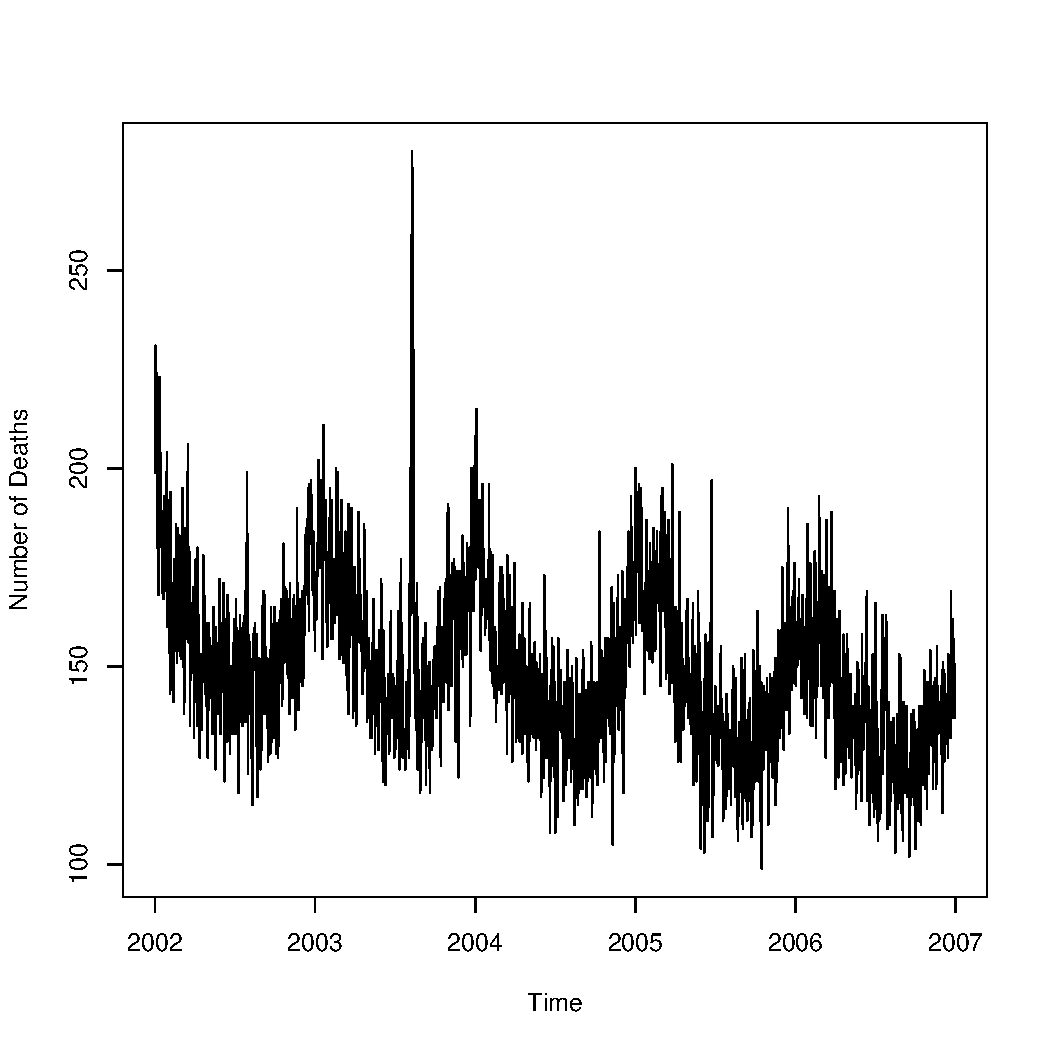
\includegraphics[width=0.50\textwidth]{figure/nn_4-1} }
\subfloat[Simulated Data\label{fig:nn_42}]{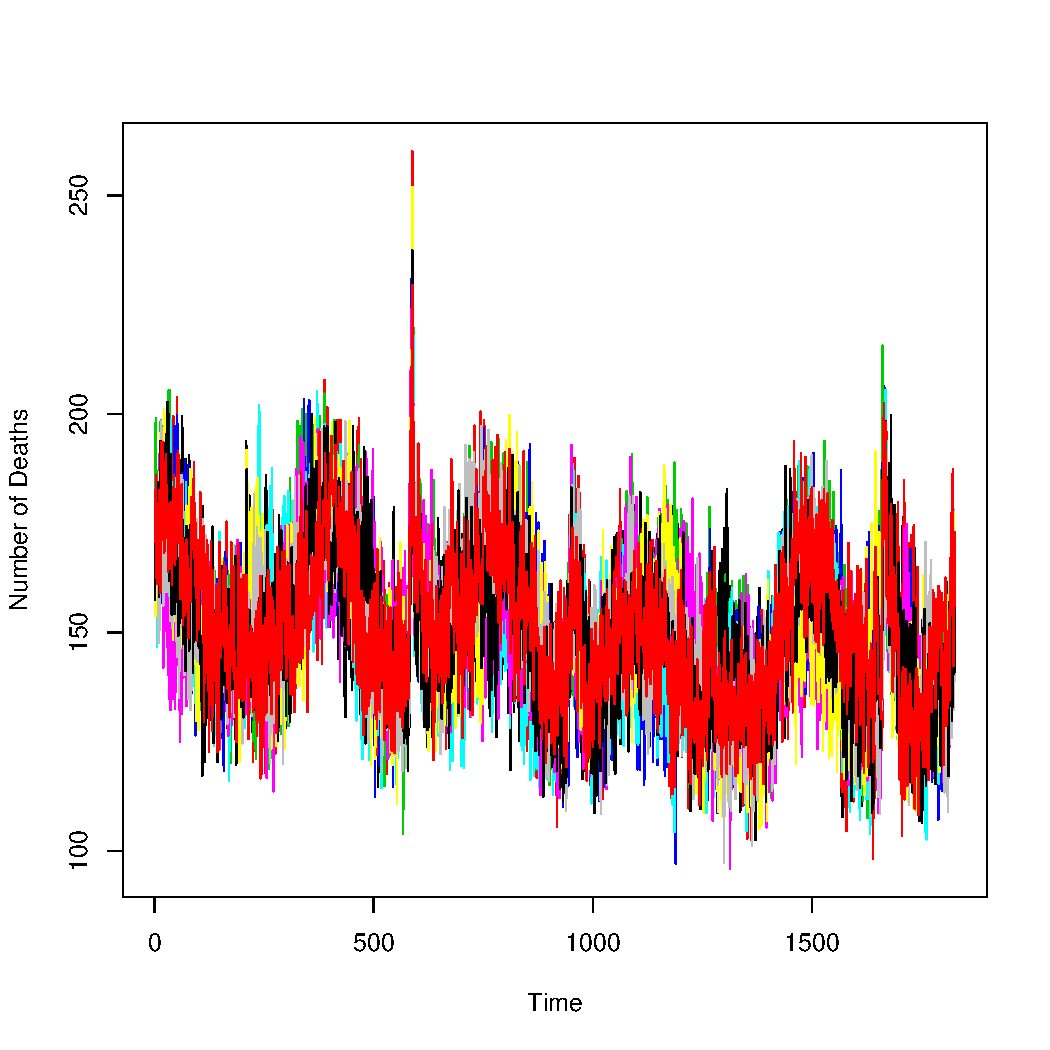
\includegraphics[width=0.50\textwidth]{figure/nn_4-2} }

}

\caption[Comparing Original Series to Simulated Data]{Comparing Original Series to Simulated Data}\label{fig:nn_4}
\end{figure}


\end{knitrout}

Unlike the other models, the NNAR model has the capability to easily simulate data.~\autoref{fig:nn_4} displays both just a few simulations and the original observed series in full. Based on these two plots, it sound to say that the observed data might come from whatever distribution the Neural Network black box is generating. This is more evidence that the generalizability of the model is quite good.

\section{Discussion} \label{s:discussion}
In this analysis, we fit three model for the time series data to predict the number of deaths, using time, ozone levels, relative humidity, temperature and temperature$^2$. The three models that we fit are time series regression, Vector autoregression and Neural Network autoregression. 

For time series regression, we first fit a linear regression using OLS, and fit two ARIMA models for the residuals, using ACF/PACF plots and auto.arima respectively. We then refit the regression model, assuming that the residuals follow the ARIMA models, and examine the fit of the new model. When comparing the results from the two approaches, we see that they do an equally good job in model fitting, residual plots, Q-Q plots, and ACF/PACF plots. Therefore, we choose the model with lower order of MA and AR. The final ARIMA model shows a moderately good forecasting behaviour, capturing the overall trend, daily volatility, but it fails to predict the correct seasonality. This model also showed that there is some directly proportional relationship between temperature and number of deaths and an inversely proportional relationship between time and number of deaths.

For Vector autoregression, we examined two models based on the seasonality components from the EDA. They both had relatively the same fit behaviour but drastically different forecasting/prediction behaviour. Thus, we choose the less complicated model in favor of explanation. The simplier model illustrated that there is some lagged effect with temperature onto the number of deaths at time $t$.

For Neural Network autoregression, we left the fitting to the black box and we were provided a model whose predicted behaviour was mostly good and captured the overall series. However, due to the nature of this statistical learning technique there is little that can learned about the relationship between number of deaths and other series.

\autoref{tab:results} displays the AIC and MSE values for the main models of interest for this analysis. Because of how Neural Networks work it does not make much sense to calculate the AIC value so this was omitted. 

% latex table generated in R 3.4.3 by xtable 1.8-3 package
% Mon Apr 29 00:08:43 2019
\begin{table}[ht]
\centering
\begin{tabular}{rrrrr}
  \hline
 & ARIMA & VAR\$\_1\$ & VAR\$\_2\$ & NNAR \\ 
  \hline
AIC & 11928.01 & 52497.02 & 53802.00 & NA \\ 
  MSE & 372.30 & 430.24 & 411.99 & 339.42 \\ 
   \hline
\end{tabular}
\caption{Evaluation Results Across all Models} 
\label{tab:results}
\end{table}


In the future, there are several things that might be of interest for further analysis. For example, utilizing \texttt{auto.arima()} to explore other parameters for the \texttt{nnetar}, gathering other influential series that might have a relation with our response variable, such as precipitation, or number of weather related incidents, \ldots and re-examining our work with decomposed components of these series.

\section{Appendix} \label{s:appendix}

\subsection*{Preliminary Setup}
\begin{knitrout}
\definecolor{shadecolor}{rgb}{0.969, 0.969, 0.969}\color{fgcolor}\begin{kframe}
\begin{alltt}
\hlcom{# Load packages}
\hlstd{pkgs} \hlkwb{<-} \hlkwd{c}\hlstd{(}\hlstr{'xtable'}\hlstd{,} \hlstr{'astsa'}\hlstd{,} \hlstr{'vars'}\hlstd{,} \hlstr{'MTS'}\hlstd{,} \hlstr{'foreign'}\hlstd{,} \hlstr{'forecast'}\hlstd{,} \hlstr{'knitr'}\hlstd{,} \hlstr{'lubridate'}\hlstd{,} \hlstr{'dplyr'}\hlstd{,} \hlstr{'magrittr'}\hlstd{)}
\hlkwd{lapply}\hlstd{(pkgs, library,} \hlkwc{character.only}\hlstd{=T)}

\hlcom{# Load data}
\hlcom{### Custom color palette}
\hlstd{cols} \hlkwb{<-} \hlkwd{c}\hlstd{(}\hlstr{'#000000'}\hlstd{,} \hlstr{'#999999'}\hlstd{,} \hlstr{'#E69F00'}\hlstd{,} \hlstr{'#56B4E9'}\hlstd{,} \hlstr{'#009E73'}\hlstd{,}
          \hlstr{'#FF0000'}\hlstd{,} \hlstr{'#F0E442'}\hlstd{,} \hlstr{'#0072B2'}\hlstd{,} \hlstr{'#D55E00'}\hlstd{,} \hlstr{'#CC79A7'}\hlstd{)}

\hlcom{### Dataset}
\hlstd{df} \hlkwb{<-} \hlkwd{read.dta}\hlstd{(}\hlstr{'./data/ije-2012-10-0989-File003.dta'}\hlstd{)}
\hlkwd{colnames}\hlstd{(df)} \hlkwb{<-} \hlkwd{c}\hlstd{(}\hlstr{'Date'}\hlstd{,} \hlstr{'Ozone'}\hlstd{,} \hlstr{'Temperature'}\hlstd{,} \hlstr{'Relative Humidity'}\hlstd{,} \hlstr{'Num Deaths'}\hlstd{)}

\hlcom{# Combine the series into a ts object with appropriate time series labeling}
\hlstd{ts_vars} \hlkwb{<-} \hlkwd{ts}\hlstd{(df[,}\hlnum{2}\hlopt{:}\hlnum{5}\hlstd{],} \hlkwc{start}\hlstd{=}\hlkwd{c}\hlstd{(}\hlnum{2002}\hlstd{,} \hlnum{1}\hlstd{),} \hlkwc{frequency}\hlstd{=}\hlnum{365.25}\hlstd{)}

\hlcom{# Cache chunk options}
\hlstd{opts_chunk}\hlopt{$}\hlkwd{set}\hlstd{(}\hlkwc{cache}\hlstd{=T,} \hlkwc{autodep}\hlstd{=T,} \hlkwc{cache.comments}\hlstd{=F)}

\hlkwd{source}\hlstd{(}\hlstr{'./fxns.R'}\hlstd{)}
\end{alltt}
\end{kframe}
\end{knitrout}

\subsection*{Introduction}
\begin{knitrout}
\definecolor{shadecolor}{rgb}{0.969, 0.969, 0.969}\color{fgcolor}\begin{kframe}
\begin{alltt}
\hlcom{# Create a sequence of numbers}
\hlstd{tab} \hlkwb{<-} \hlkwd{t}\hlstd{(}\hlkwd{apply}\hlstd{(ts_vars,} \hlnum{2}\hlstd{, summary))}
\hlstd{xt} \hlkwb{<-} \hlkwd{xtable}\hlstd{(tab,} \hlkwc{label}\hlstd{=}\hlstr{'tab:data_summary'}\hlstd{,}
    \hlkwc{caption}\hlstd{=}\hlstr{'Summary Statistics for Individual Time Series'}\hlstd{)}
\hlkwd{print}\hlstd{(xt)}
\end{alltt}
\end{kframe}
\end{knitrout}

\subsection*{Method}
\begin{knitrout}
\definecolor{shadecolor}{rgb}{0.969, 0.969, 0.969}\color{fgcolor}\begin{kframe}
\begin{alltt}
\hlcom{# Plotting overall time series}
\hlkwd{plot.ts}\hlstd{(ts_vars,} \hlkwc{main} \hlstd{=} \hlstr{""}\hlstd{)}

\hlcom{# Determining seasonality component}
\hlstd{seasonal} \hlkwb{=} \hlkwd{lapply}\hlstd{(df[,}\hlnum{2}\hlopt{:}\hlnum{5}\hlstd{],} \hlkwa{function}\hlstd{(}\hlkwc{x}\hlstd{,} \hlkwc{vars}\hlstd{) \{}
  \hlstd{x} \hlkwb{<-} \hlkwd{ts}\hlstd{(x,} \hlkwc{start}\hlstd{=}\hlkwd{c}\hlstd{(}\hlnum{2002}\hlstd{,} \hlnum{1}\hlstd{),} \hlkwc{frequency}\hlstd{=}\hlnum{365}\hlstd{)}
  \hlstd{temp} \hlkwb{<-} \hlkwd{decompose}\hlstd{(x)}
  \hlkwd{return}\hlstd{(temp}\hlopt{$}\hlstd{seasonal)}
\hlstd{\})}

\hlcom{# Plotting seasonality componen}
\hlkwd{plot.ts}\hlstd{(}\hlkwd{do.call}\hlstd{(cbind, seasonal),} \hlkwc{main} \hlstd{=} \hlstr{''}\hlstd{)}
\end{alltt}
\end{kframe}
\end{knitrout}
\begin{knitrout}
\definecolor{shadecolor}{rgb}{0.969, 0.969, 0.969}\color{fgcolor}\begin{kframe}
\begin{alltt}
\hlcom{# pairs plot of all series}
\hlkwd{pairs}\hlstd{(ts_vars,} \hlkwc{cex}\hlstd{=}\hlnum{0.75}\hlstd{,} \hlkwc{pch}\hlstd{=}\hlnum{16}\hlstd{)}
\end{alltt}
\end{kframe}
\end{knitrout}

\begin{knitrout}
\definecolor{shadecolor}{rgb}{0.969, 0.969, 0.969}\color{fgcolor}\begin{kframe}
\begin{alltt}
\hlcom{# Variable transformation indicated by EDA}
\hlstd{df} \hlopt
  \hlkwd{mutate}\hlstd{(}\hlkwc{`Adjusted Temperature`} \hlstd{= Temperature} \hlopt{-} \hlkwd{mean}\hlstd{(Temperature),}
         \hlkwc{`(Adjusted Temperature)^2`} \hlstd{= `Adjusted Temperature`}\hlopt{^}\hlnum{2}\hlstd{,}
         \hlkwc{`Day of Week`} \hlstd{= lubridate}\hlopt{::}\hlkwd{wday}\hlstd{(Date),}
         \hlkwc{`Day of Month`} \hlstd{= lubridate}\hlopt{::}\hlkwd{mday}\hlstd{(Date))}

\hlstd{ts_vars} \hlkwb{<-} \hlkwd{ts}\hlstd{(df[,}\hlkwd{c}\hlstd{(}\hlnum{2}\hlstd{,} \hlnum{6}\hlopt{:}\hlnum{7}\hlstd{,} \hlnum{4}\hlopt{:}\hlnum{5}\hlstd{,} \hlnum{8}\hlopt{:}\hlnum{9}\hlstd{)],} \hlkwc{start}\hlstd{=}\hlkwd{c}\hlstd{(}\hlnum{2002}\hlstd{,} \hlnum{1}\hlstd{),} \hlkwc{frequency}\hlstd{=}\hlnum{365.25}\hlstd{)}

\hlcom{# Formulate training/testing split where testing is 1 year}
\hlstd{train} \hlkwb{<-} \hlkwd{window}\hlstd{(ts_vars,} \hlkwc{start}\hlstd{=}\hlkwd{c}\hlstd{(}\hlnum{2002}\hlstd{,} \hlnum{1}\hlstd{),} \hlkwc{end}\hlstd{=}\hlkwd{c}\hlstd{(}\hlnum{2005}\hlstd{,} \hlnum{365.25}\hlstd{))}
\hlstd{test} \hlkwb{<-} \hlkwd{window}\hlstd{(ts_vars,} \hlkwc{start}\hlstd{=}\hlkwd{c}\hlstd{(}\hlnum{2006}\hlstd{,} \hlnum{1}\hlstd{))}
\hlstd{train_trend} \hlkwb{=} \hlkwd{time}\hlstd{(train); test_trend} \hlkwb{=} \hlkwd{time}\hlstd{(test)}

\hlstd{results} \hlkwb{<-} \hlkwd{matrix}\hlstd{(}\hlnum{0}\hlstd{,} \hlkwc{nrow}\hlstd{=}\hlnum{2}\hlstd{,} \hlkwc{ncol}\hlstd{=}\hlnum{4}\hlstd{,}
  \hlkwc{dimnames}\hlstd{=}\hlkwd{list}\hlstd{(}\hlkwd{c}\hlstd{(}\hlstr{'AIC'}\hlstd{,} \hlstr{'MSE'}\hlstd{),}
    \hlkwd{c}\hlstd{(}\hlstr{'ARIMA'}\hlstd{,} \hlstr{'VAR$_1$'}\hlstd{,} \hlstr{'VAR$_2$'}\hlstd{,} \hlstr{'NNAR'}\hlstd{)))}
\end{alltt}
\end{kframe}
\end{knitrout}
\begin{knitrout}
\definecolor{shadecolor}{rgb}{0.969, 0.969, 0.969}\color{fgcolor}\begin{kframe}
\begin{alltt}
\hlcom{# Fit `lm()` to exogenous variables to determine ARIMA fit}
\hlcom{# Fit `lm()` to exogenous variables to determine ARIMA fit}
\hlstd{ts_reg_1} \hlkwb{=} \hlkwd{lm}\hlstd{(train[,}\hlstr{'Num Deaths'}\hlstd{]} \hlopt{~} \hlstd{train_trend} \hlopt{+} \hlstd{train[,}\hlstr{'Ozone'}\hlstd{]} \hlopt{+}
  \hlstd{train[,}\hlstr{'Adjusted Temperature'}\hlstd{]} \hlopt{+} \hlstd{train[,}\hlstr{'(Adjusted Temperature)^2'}\hlstd{]} \hlopt{+}
  \hlstd{train[,}\hlstr{'Relative Humidity'}\hlstd{]} \hlopt{+} \hlstd{train[,}\hlstr{'Day of Week'}\hlstd{]} \hlopt{+} \hlstd{train[,}\hlstr{'Day of Month'}\hlstd{])}

\hlcom{# Looking at residuals}
\hlkwd{plot}\hlstd{(}\hlkwd{resid}\hlstd{(ts_reg_1),} \hlkwc{ylab}\hlstd{=}\hlstr{'Residuals'}\hlstd{,} \hlkwc{cex}\hlstd{=}\hlnum{0.75}\hlstd{)}
\hlkwd{abline}\hlstd{(}\hlkwc{h}\hlstd{=}\hlnum{0}\hlstd{,} \hlkwc{col}\hlstd{=}\hlstr{'red'}\hlstd{,} \hlkwc{lwd}\hlstd{=}\hlnum{2}\hlstd{)}
\hlkwd{qqnorm}\hlstd{(}\hlkwd{resid}\hlstd{(ts_reg_1));} \hlkwd{qqline}\hlstd{(}\hlkwd{resid}\hlstd{(ts_reg_1))}
\end{alltt}
\end{kframe}
\end{knitrout}
\begin{knitrout}
\definecolor{shadecolor}{rgb}{0.969, 0.969, 0.969}\color{fgcolor}\begin{kframe}
\begin{alltt}
\hlcom{# Looking at ACF/PACF for model identification}
\hlkwd{invisible}\hlstd{(astsa}\hlopt{::}\hlkwd{acf2}\hlstd{(}\hlkwd{resid}\hlstd{(ts_reg_1),} \hlnum{365.25}\hlstd{,} \hlkwc{main}\hlstd{=}\hlstr{''}\hlstd{))}
\end{alltt}
\end{kframe}
\end{knitrout}
\begin{knitrout}
\definecolor{shadecolor}{rgb}{0.969, 0.969, 0.969}\color{fgcolor}\begin{kframe}
\begin{alltt}
\hlcom{###### Parameter selection}
\hlstd{train_var} \hlkwb{<-} \hlstd{train[,}\hlkwd{c}\hlstd{(}\hlstr{'Ozone'}\hlstd{,} \hlstr{'Adjusted Temperature'}\hlstd{,} \hlstr{'(Adjusted Temperature)^2'}\hlstd{,}
  \hlstr{'Relative Humidity'}\hlstd{,} \hlstr{'Num Deaths'}\hlstd{)]}
\hlstd{bind} \hlkwb{<-} \hlkwd{cbind}\hlstd{(}\hlkwc{trend}\hlstd{=train_trend,} \hlkwc{wday}\hlstd{=train[,}\hlstr{'Day of Week'}\hlstd{],} \hlkwc{mday}\hlstd{=train[,}\hlstr{'Day of Month'}\hlstd{])}

\hlcom{# Calculate Information Criteria for different VAR(p) models with season=NULL}
\hlstd{VARselect_res_1} \hlkwb{<-} \hlkwd{VARselect}\hlstd{(train_var,} \hlkwc{season}\hlstd{=}\hlkwa{NULL}\hlstd{,} \hlkwc{exogen}\hlstd{=bind,} \hlkwc{type}\hlstd{=}\hlstr{'none'}\hlstd{)}

\hlcom{# Calculate Information Criteria for different VAR(p) models with season=365}
\hlstd{VARselect_res_2} \hlkwb{<-} \hlkwd{VARselect}\hlstd{(train_var,} \hlkwc{season}\hlstd{=}\hlnum{365}\hlstd{,} \hlkwc{exogen}\hlstd{=bind,} \hlkwc{type}\hlstd{=}\hlstr{'none'}\hlstd{)}

\hlstd{selection} \hlkwb{<-} \hlkwd{rbind}\hlstd{(VARselect_res_1}\hlopt{$}\hlstd{selection, VARselect_res_2}\hlopt{$}\hlstd{selection)}
\hlkwd{rownames}\hlstd{(selection)} \hlkwb{<-} \hlkwd{paste0}\hlstd{(}\hlstr{'season='}\hlstd{,} \hlkwd{c}\hlstd{(}\hlstr{'NULL'}\hlstd{,} \hlstr{'365'}\hlstd{))}
\hlstd{xt} \hlkwb{<-} \hlkwd{xtable}\hlstd{(selection,} \hlkwc{label}\hlstd{=}\hlstr{'tab:var_order'}\hlstd{,}
  \hlkwc{caption}\hlstd{=}\hlstr{'\textbackslash{}\textbackslash{}texttt\{VARselect()\} Order Selection for Different Models'}\hlstd{)}
\hlkwd{print}\hlstd{(xt,} \hlkwc{table.placement}\hlstd{=}\hlstr{'H'}\hlstd{)}
\end{alltt}
\end{kframe}
\end{knitrout}

\subsection*{Results}
\subsubsection*{Time Series Regression}
\begin{knitrout}
\definecolor{shadecolor}{rgb}{0.969, 0.969, 0.969}\color{fgcolor}\begin{kframe}
\begin{alltt}
\hlcom{# Fit `Arima()` to residuals of exogenous variables}
\hlstd{bind} \hlkwb{<-} \hlkwd{cbind}\hlstd{(}\hlkwc{trend}\hlstd{=train_trend,} \hlkwc{temp}\hlstd{=train[,}\hlstr{'Adjusted Temperature'}\hlstd{],}
  \hlkwc{temp2}\hlstd{=train[,}\hlstr{'(Adjusted Temperature)^2'}\hlstd{],} \hlkwc{Ozone}\hlstd{=train[,}\hlstr{'Ozone'}\hlstd{],}
  \hlkwc{`Relative Humidity`}\hlstd{=train[,}\hlstr{'Relative Humidity'}\hlstd{],} \hlkwc{wday}\hlstd{=train[,}\hlstr{'Day of Week'}\hlstd{],}
  \hlkwc{mday}\hlstd{=train[,}\hlstr{'Day of Month'}\hlstd{])}
\hlstd{ts_reg_2} \hlkwb{=} \hlkwd{Arima}\hlstd{(train[,}\hlstr{'Num Deaths'}\hlstd{],} \hlkwc{order}\hlstd{=}\hlkwd{c}\hlstd{(}\hlnum{2}\hlstd{,} \hlnum{0}\hlstd{,} \hlnum{8}\hlstd{),} \hlkwc{xreg}\hlstd{=bind,} \hlkwc{optim.control}\hlstd{=}\hlkwd{list}\hlstd{(}\hlkwc{maxit}\hlstd{=}\hlnum{1000}\hlstd{))}

\hlcom{# Looking at fitted values}
\hlkwd{plot}\hlstd{(train[,}\hlstr{'Num Deaths'}\hlstd{],} \hlkwc{ylab}\hlstd{=}\hlstr{'Number of Deaths'}\hlstd{)}
\hlkwd{lines}\hlstd{(}\hlkwd{fitted}\hlstd{(ts_reg_2),} \hlkwc{col}\hlstd{=}\hlstr{'blue'}\hlstd{)}
\hlkwd{legend}\hlstd{(}\hlstr{'topright'}\hlstd{,} \hlkwd{c}\hlstd{(}\hlstr{'Original Data'}\hlstd{,} \hlstr{'Fitted Values'}\hlstd{),} \hlkwc{lty}\hlstd{=}\hlkwd{c}\hlstd{(}\hlnum{1}\hlstd{,}\hlnum{1}\hlstd{),} \hlkwc{col}\hlstd{=}\hlkwd{c}\hlstd{(}\hlnum{1}\hlstd{,}\hlstr{'blue'}\hlstd{))}

\hlcom{# Looking at residuals over time}
\hlkwd{plot}\hlstd{(}\hlkwd{resid}\hlstd{(ts_reg_2),} \hlkwc{ylab}\hlstd{=}\hlstr{'Residuals'}\hlstd{,} \hlkwc{type}\hlstd{=}\hlstr{'p'}\hlstd{,} \hlkwc{cex}\hlstd{=}\hlnum{0.75}\hlstd{)}
\hlkwd{abline}\hlstd{(}\hlkwc{h}\hlstd{=}\hlnum{0}\hlstd{,} \hlkwc{col}\hlstd{=}\hlstr{'red'}\hlstd{,} \hlkwc{lwd}\hlstd{=}\hlnum{2}\hlstd{)}
\end{alltt}
\end{kframe}
\end{knitrout}
\begin{knitrout}
\definecolor{shadecolor}{rgb}{0.969, 0.969, 0.969}\color{fgcolor}\begin{kframe}
\begin{alltt}
\hlcom{# Fit `Arima()` to residuals of exogenous variables}
\hlstd{ts_reg_3} \hlkwb{=} \hlkwd{auto.arima}\hlstd{(train[,} \hlstr{'Num Deaths'}\hlstd{],} \hlkwc{xreg}\hlstd{=bind,} \hlkwc{seasonal}\hlstd{=T,}
  \hlkwc{stepwise}\hlstd{=F,} \hlkwc{approximation}\hlstd{=F,} \hlkwc{optim.control}\hlstd{=}\hlkwd{list}\hlstd{(}\hlkwc{maxit}\hlstd{=}\hlnum{1000}\hlstd{))}

\hlcom{# Looking at fitted values}
\hlkwd{plot}\hlstd{(train[,} \hlstr{'Num Deaths'}\hlstd{],} \hlkwc{ylab}\hlstd{=}\hlstr{'Number of Deaths'}\hlstd{)}
\hlkwd{lines}\hlstd{(}\hlkwd{fitted}\hlstd{(ts_reg_3),} \hlkwc{col}\hlstd{=}\hlstr{'blue'}\hlstd{)}
\hlkwd{legend}\hlstd{(}\hlstr{'topright'}\hlstd{,} \hlkwd{c}\hlstd{(}\hlstr{'Original Data'}\hlstd{,} \hlstr{'Fitted Values'}\hlstd{),} \hlkwc{lty}\hlstd{=}\hlkwd{c}\hlstd{(}\hlnum{1}\hlstd{,}\hlnum{1}\hlstd{),} \hlkwc{col}\hlstd{=}\hlkwd{c}\hlstd{(}\hlnum{1}\hlstd{,}\hlstr{'blue'}\hlstd{))}

\hlcom{# Looking at residuals over time}
\hlkwd{plot}\hlstd{(}\hlkwd{resid}\hlstd{(ts_reg_3),} \hlkwc{type}\hlstd{=}\hlstr{'p'}\hlstd{,} \hlkwc{cex}\hlstd{=}\hlnum{0.75}\hlstd{,} \hlkwc{ylab} \hlstd{=} \hlstr{'Residuals'}\hlstd{)}
\hlkwd{abline}\hlstd{(}\hlkwc{h}\hlstd{=}\hlnum{0}\hlstd{,} \hlkwc{col}\hlstd{=}\hlstr{'red'}\hlstd{,} \hlkwc{lwd}\hlstd{=}\hlnum{2}\hlstd{)}
\end{alltt}
\end{kframe}
\end{knitrout}
\begin{knitrout}
\definecolor{shadecolor}{rgb}{0.969, 0.969, 0.969}\color{fgcolor}\begin{kframe}
\begin{alltt}
\hlcom{# Looking at normality of residuals}
\hlkwd{qqnorm}\hlstd{(}\hlkwd{resid}\hlstd{(ts_reg_2));} \hlkwd{qqline}\hlstd{(}\hlkwd{resid}\hlstd{(ts_reg_2))}

\hlcom{# Looking at ACF/PACF for white noise}
\hlkwd{invisible}\hlstd{(astsa}\hlopt{::}\hlkwd{acf2}\hlstd{(}\hlkwd{resid}\hlstd{(ts_reg_2),} \hlnum{365.25}\hlstd{,} \hlkwc{main}\hlstd{=}\hlstr{''}\hlstd{))}
\end{alltt}
\end{kframe}
\end{knitrout}
\begin{knitrout}
\definecolor{shadecolor}{rgb}{0.969, 0.969, 0.969}\color{fgcolor}\begin{kframe}
\begin{alltt}
\hlcom{# Looking at normality of residuals}
\hlkwd{qqnorm}\hlstd{(}\hlkwd{resid}\hlstd{(ts_reg_3));} \hlkwd{qqline}\hlstd{(}\hlkwd{resid}\hlstd{(ts_reg_3))}

\hlcom{# Looking at ACF/PACF for white noise}
\hlkwd{invisible}\hlstd{(}\hlkwd{acf2}\hlstd{(}\hlkwd{resid}\hlstd{(ts_reg_3),} \hlnum{365.25}\hlstd{,} \hlkwc{main}\hlstd{=}\hlstr{''}\hlstd{))}
\end{alltt}
\end{kframe}
\end{knitrout}
\begin{knitrout}
\definecolor{shadecolor}{rgb}{0.969, 0.969, 0.969}\color{fgcolor}\begin{kframe}
\begin{alltt}
\hlcom{###### Forecasting test data}
\hlstd{bind} \hlkwb{<-} \hlkwd{cbind}\hlstd{(}\hlkwc{trend}\hlstd{=test_trend,} \hlkwc{temp}\hlstd{=test[,} \hlstr{'Adjusted Temperature'}\hlstd{],}
  \hlkwc{temp2}\hlstd{=test[,} \hlstr{'(Adjusted Temperature)^2'}\hlstd{],} \hlkwc{Ozone}\hlstd{=test[,} \hlstr{'Ozone'}\hlstd{],}
  \hlkwc{`Relative Humidity`}\hlstd{=test[,}\hlstr{'Relative Humidity'}\hlstd{],} \hlkwc{wday}\hlstd{=test[,}\hlstr{'Day of Week'}\hlstd{],}
  \hlkwc{mday}\hlstd{=test[,}\hlstr{'Day of Month'}\hlstd{])}
\hlstd{fcast} \hlkwb{<-} \hlkwd{forecast}\hlstd{(ts_reg_3,} \hlkwc{level}\hlstd{=}\hlnum{95}\hlstd{,} \hlkwc{xreg}\hlstd{=bind)}

\hlkwd{plot}\hlstd{(train[,} \hlstr{'Num Deaths'}\hlstd{],} \hlkwc{ylab}\hlstd{=}\hlstr{'Number of Deaths'}\hlstd{,} \hlkwc{xlim}\hlstd{=}\hlkwd{c}\hlstd{(}\hlnum{2002}\hlstd{,} \hlnum{2007}\hlstd{),}
  \hlkwc{ylim}\hlstd{=}\hlkwd{range}\hlstd{(fcast}\hlopt{$}\hlstd{lower, fcast}\hlopt{$}\hlstd{upper, ts_vars[,} \hlstr{'Num Deaths'}\hlstd{]))}
\hlkwd{lines}\hlstd{(test[,} \hlstr{'Num Deaths'}\hlstd{],} \hlkwc{col} \hlstd{=} \hlstr{'darkgrey'}\hlstd{)}
\hlkwd{lines}\hlstd{(fcast}\hlopt{$}\hlstd{upper,} \hlkwc{col} \hlstd{=} \hlstr{'red'}\hlstd{,} \hlkwc{lty} \hlstd{=} \hlnum{2}\hlstd{)}
\hlkwd{lines}\hlstd{(fcast}\hlopt{$}\hlstd{mean,} \hlkwc{col} \hlstd{=} \hlstr{'red'}\hlstd{)}
\hlkwd{lines}\hlstd{(fcast}\hlopt{$}\hlstd{lower,} \hlkwc{col} \hlstd{=} \hlstr{'red'}\hlstd{,} \hlkwc{lty} \hlstd{=} \hlnum{2}\hlstd{)}
\hlkwd{legend}\hlstd{(}\hlstr{'topright'}\hlstd{,} \hlkwd{c}\hlstd{(}\hlstr{'Training Data'}\hlstd{,} \hlstr{'Validation Data'}\hlstd{,} \hlstr{'Point Estimates'}\hlstd{,} \hlstr{'95% CI'}\hlstd{),}
  \hlkwc{col}\hlstd{=}\hlkwd{c}\hlstd{(}\hlnum{1}\hlstd{,} \hlstr{'grey'}\hlstd{,} \hlstr{'red'}\hlstd{,} \hlstr{'red'}\hlstd{),} \hlkwc{lty}\hlstd{=}\hlkwd{c}\hlstd{(}\hlnum{1}\hlstd{,}\hlnum{1}\hlstd{,}\hlnum{1}\hlstd{,}\hlnum{2}\hlstd{),} \hlkwc{cex}\hlstd{=}\hlnum{0.75}\hlstd{)}
\end{alltt}
\end{kframe}
\end{knitrout}
\begin{knitrout}
\definecolor{shadecolor}{rgb}{0.969, 0.969, 0.969}\color{fgcolor}\begin{kframe}
\begin{alltt}
\hlcom{# Display coefficients and standard errors}
\hlstd{output} \hlkwb{<-} \hlkwd{capture.output}\hlstd{(ts_reg_3)}
\hlstd{output} \hlkwb{<-} \hlkwd{strsplit}\hlstd{(output,} \hlstr{'( *: )|[ ]\{2,\}'}\hlstd{,} \hlkwc{perl}\hlstd{=}\hlnum{TRUE}\hlstd{)}
\hlstd{output} \hlkwb{<-} \hlstd{output[}\hlnum{5}\hlopt{:}\hlnum{10}\hlstd{]}
\hlstd{output} \hlkwb{<-} \hlkwd{cbind}\hlstd{(}\hlkwd{do.call}\hlstd{(rbind, output[}\hlnum{1}\hlopt{:}\hlnum{3}\hlstd{]),} \hlkwd{do.call}\hlstd{(rbind, output[}\hlnum{4}\hlopt{:}\hlnum{6}\hlstd{]))}
\hlstd{tab} \hlkwb{<-} \hlkwd{apply}\hlstd{(output[}\hlopt{-}\hlnum{1}\hlstd{,}\hlopt{-}\hlkwd{c}\hlstd{(}\hlnum{1}\hlstd{,}\hlnum{9}\hlstd{)],} \hlnum{1}\hlstd{, as.numeric)}
\hlkwd{rownames}\hlstd{(tab)} \hlkwb{<-} \hlkwd{c}\hlstd{(}\hlstr{'ar 1'}\hlstd{,} \hlstr{'ma 1'}\hlstd{,} \hlstr{'intercept'}\hlstd{,} \hlstr{'Trend'}\hlstd{,} \hlkwd{colnames}\hlstd{(ts_vars)[}\hlkwd{c}\hlstd{(}\hlnum{2}\hlopt{:}\hlnum{3}\hlstd{,} \hlnum{1}\hlstd{,} \hlnum{4}\hlstd{,} \hlnum{6}\hlopt{:}\hlnum{7}\hlstd{)])}
\hlkwd{rownames}\hlstd{(tab)[}\hlnum{6}\hlstd{]} \hlkwb{<-} \hlstr{'(Adjusted Temperature)$^2$'}
\hlkwd{colnames}\hlstd{(tab)} \hlkwb{<-} \hlkwd{c}\hlstd{(}\hlstr{'Estimate'}\hlstd{,} \hlstr{'Std. Error'}\hlstd{)}
\hlstd{xt} \hlkwb{<-} \hlkwd{xtable}\hlstd{(tab,} \hlkwc{caption}\hlstd{=}\hlstr{'Time Series Estimated Coefficients'}\hlstd{,} \hlkwc{label}\hlstd{=}\hlstr{'tab:ts_reg'}\hlstd{,} \hlkwc{digits}\hlstd{=}\hlnum{2}\hlstd{)}
\hlkwd{print}\hlstd{(xt,} \hlkwc{scalebox}\hlstd{=}\hlnum{1}\hlstd{,} \hlkwc{sanitize.rownames.function} \hlstd{=} \hlkwa{function}\hlstd{(}\hlkwc{x}\hlstd{) \{x\})}

\hlcom{# Calculate final results for model}
\hlstd{results[,}\hlstr{'ARIMA'}\hlstd{]} \hlkwb{<-} \hlkwd{c}\hlstd{(}\hlkwd{AIC}\hlstd{(ts_reg_3),} \hlkwd{mean}\hlstd{((test[,}\hlstr{'Num Deaths'}\hlstd{]} \hlopt{-} \hlstd{fcast}\hlopt{$}\hlstd{mean)}\hlopt{^}\hlnum{2}\hlstd{))}
\end{alltt}
\end{kframe}
\end{knitrout}

\subsubsection*{Vector Autoregression}
\begin{knitrout}
\definecolor{shadecolor}{rgb}{0.969, 0.969, 0.969}\color{fgcolor}\begin{kframe}
\begin{alltt}
\hlcom{# Determining VAR model based on VARselect_res_1}
\hlstd{bind} \hlkwb{<-} \hlkwd{cbind}\hlstd{(}\hlkwc{trend}\hlstd{=train_trend,} \hlkwc{wday}\hlstd{=train[,}\hlstr{'Day of Week'}\hlstd{],} \hlkwc{mday}\hlstd{=train[,}\hlstr{'Day of Month'}\hlstd{])}
\hlstd{var_fit_1} \hlkwb{<-} \hlstd{vars}\hlopt{::}\hlkwd{VAR}\hlstd{(train_var,} \hlkwc{p}\hlstd{=}\hlkwd{min}\hlstd{(selection[}\hlnum{1}\hlstd{,]),}
  \hlkwc{season}\hlstd{=}\hlkwa{NULL}\hlstd{,} \hlkwc{exogen}\hlstd{=bind,} \hlkwc{type}\hlstd{=}\hlstr{'none'}\hlstd{)}

\hlcom{# Display fitted values and original series}
\hlstd{ts_fitted} \hlkwb{<-} \hlkwd{ts}\hlstd{(}\hlkwd{fitted}\hlstd{(var_fit_1),} \hlkwc{start}\hlstd{=}\hlkwd{c}\hlstd{(}\hlnum{2002}\hlstd{,} \hlnum{1}\hlstd{),} \hlkwc{frequency}\hlstd{=}\hlnum{365.25}\hlstd{)}
\hlkwd{temp_plot}\hlstd{(train_var,} \hlkwc{other}\hlstd{=ts_fitted,} \hlkwc{other_col}\hlstd{=}\hlstr{'blue'}\hlstd{,} \hlkwc{main}\hlstd{=}\hlstr{''}\hlstd{)}

\hlcom{# Display residuals over time}
\hlstd{ts_resid_1} \hlkwb{<-} \hlkwd{ts}\hlstd{(}\hlkwd{resid}\hlstd{(var_fit_1),} \hlkwc{start}\hlstd{=}\hlkwd{c}\hlstd{(}\hlnum{2002}\hlstd{,} \hlnum{1}\hlstd{),} \hlkwc{frequency}\hlstd{=}\hlnum{365.25}\hlstd{)}
\hlkwd{colnames}\hlstd{(ts_resid_1)} \hlkwb{<-} \hlkwd{colnames}\hlstd{(train_var)}
\hlstd{ts_line} \hlkwb{<-} \hlkwd{ts}\hlstd{(}\hlkwd{matrix}\hlstd{(}\hlnum{0}\hlstd{,} \hlkwc{ncol}\hlstd{=}\hlkwd{ncol}\hlstd{(train_var),} \hlkwc{nrow}\hlstd{=}\hlkwd{nrow}\hlstd{(train)),} \hlkwc{start}\hlstd{=}\hlkwd{c}\hlstd{(}\hlnum{2002}\hlstd{,}\hlnum{1}\hlstd{),} \hlkwc{frequency}\hlstd{=}\hlnum{365.25}\hlstd{)}
\hlkwd{temp_plot}\hlstd{(ts_resid_1,} \hlkwc{other}\hlstd{=ts_line,} \hlkwc{other_col}\hlstd{=}\hlstr{'red'}\hlstd{,} \hlkwc{main}\hlstd{=}\hlstr{''}\hlstd{)}
\end{alltt}
\end{kframe}
\end{knitrout}
\begin{knitrout}
\definecolor{shadecolor}{rgb}{0.969, 0.969, 0.969}\color{fgcolor}\begin{kframe}
\begin{alltt}
\hlcom{# Determining VAR model based on VARselect_res_2}
\hlstd{var_fit_2} \hlkwb{<-} \hlstd{vars}\hlopt{::}\hlkwd{VAR}\hlstd{(train_var,} \hlkwc{p}\hlstd{=}\hlkwd{min}\hlstd{(selection[}\hlnum{2}\hlstd{,]),}
  \hlkwc{season}\hlstd{=}\hlnum{365}\hlstd{,} \hlkwc{exogen}\hlstd{=bind,} \hlkwc{type}\hlstd{=}\hlstr{'none'}\hlstd{)}

\hlcom{# Display fitted values and original series}
\hlstd{ts_fitted} \hlkwb{<-} \hlkwd{ts}\hlstd{(}\hlkwd{fitted}\hlstd{(var_fit_2),} \hlkwc{start}\hlstd{=}\hlkwd{c}\hlstd{(}\hlnum{2002}\hlstd{,} \hlnum{1}\hlstd{),} \hlkwc{frequency}\hlstd{=}\hlnum{365.25}\hlstd{)}
\hlkwd{temp_plot}\hlstd{(train_var,} \hlkwc{other}\hlstd{=ts_fitted,} \hlkwc{other_col}\hlstd{=}\hlstr{'blue'}\hlstd{,} \hlkwc{main}\hlstd{=}\hlstr{''}\hlstd{)}

\hlcom{# Display residuals over time}
\hlstd{ts_resid_2} \hlkwb{<-} \hlkwd{ts}\hlstd{(}\hlkwd{resid}\hlstd{(var_fit_2),} \hlkwc{start}\hlstd{=}\hlkwd{c}\hlstd{(}\hlnum{2002}\hlstd{,} \hlnum{1}\hlstd{),} \hlkwc{frequency}\hlstd{=}\hlnum{365.25}\hlstd{)}
\hlkwd{colnames}\hlstd{(ts_resid_2)} \hlkwb{<-} \hlkwd{colnames}\hlstd{(train_var)}
\hlstd{ts_line} \hlkwb{<-} \hlkwd{ts}\hlstd{(}\hlkwd{matrix}\hlstd{(}\hlnum{0}\hlstd{,} \hlkwc{ncol}\hlstd{=}\hlkwd{ncol}\hlstd{(train_var),} \hlkwc{nrow}\hlstd{=}\hlkwd{nrow}\hlstd{(train)),} \hlkwc{start}\hlstd{=}\hlkwd{c}\hlstd{(}\hlnum{2002}\hlstd{,}\hlnum{1}\hlstd{),} \hlkwc{frequency}\hlstd{=}\hlnum{365.25}\hlstd{)}
\hlkwd{temp_plot}\hlstd{(ts_resid_2,} \hlkwc{other}\hlstd{=ts_line,} \hlkwc{other_col}\hlstd{=}\hlstr{'red'}\hlstd{,} \hlkwc{main}\hlstd{=}\hlstr{''}\hlstd{)}
\end{alltt}
\end{kframe}
\end{knitrout}
\begin{knitrout}
\definecolor{shadecolor}{rgb}{0.969, 0.969, 0.969}\color{fgcolor}\begin{kframe}
\begin{alltt}
\hlcom{# Display ACF/CCF plots}
\hlkwd{acf}\hlstd{(ts_resid_1,} \hlkwc{lag.max}\hlstd{=}\hlnum{365.25}\hlstd{,} \hlkwc{mar}\hlstd{=}\hlkwd{c}\hlstd{(}\hlnum{2.85}\hlstd{,} \hlnum{2.5}\hlstd{,} \hlnum{2}\hlstd{,} \hlnum{0.25}\hlstd{))}
\hlkwd{acf}\hlstd{(ts_resid_2,} \hlkwc{lag.max}\hlstd{=}\hlnum{365.25}\hlstd{,} \hlkwc{mar}\hlstd{=}\hlkwd{c}\hlstd{(}\hlnum{2.85}\hlstd{,} \hlnum{2.5}\hlstd{,} \hlnum{2}\hlstd{,} \hlnum{0.25}\hlstd{))}
\end{alltt}
\end{kframe}
\end{knitrout}
\begin{knitrout}
\definecolor{shadecolor}{rgb}{0.969, 0.969, 0.969}\color{fgcolor}\begin{kframe}
\begin{alltt}
\hlcom{# Forecasting VAR(season=NULL)}
\hlstd{bind} \hlkwb{<-} \hlkwd{cbind}\hlstd{(}\hlkwc{trend}\hlstd{=test_trend,} \hlkwc{wday}\hlstd{=test[,}\hlstr{'Day of Week'}\hlstd{],} \hlkwc{mday}\hlstd{=test[,}\hlstr{'Day of Month'}\hlstd{])}
\hlstd{fcast} \hlkwb{<-} \hlkwd{predict}\hlstd{(var_fit_1,} \hlkwc{n.ahead}\hlstd{=}\hlkwd{nrow}\hlstd{(test),} \hlkwc{dumvar}\hlstd{=bind)}
\hlkwd{names}\hlstd{(fcast}\hlopt{$}\hlstd{fcst)} \hlkwb{<-} \hlkwd{colnames}\hlstd{(train_var)}
\hlkwd{colnames}\hlstd{(fcast}\hlopt{$}\hlstd{endog)} \hlkwb{<-} \hlkwd{colnames}\hlstd{(train_var)}

\hlkwd{plot}\hlstd{(train[,} \hlstr{'Num Deaths'}\hlstd{],} \hlkwc{ylab}\hlstd{=}\hlstr{'Number of Deaths'}\hlstd{,} \hlkwc{xlim} \hlstd{=} \hlkwd{c}\hlstd{(}\hlnum{2002}\hlstd{,} \hlnum{2007}\hlstd{),}
  \hlkwc{ylim}\hlstd{=}\hlkwd{range}\hlstd{(fcast}\hlopt{$}\hlstd{fcst}\hlopt{$}\hlstd{`Num Deaths`[,} \hlnum{1}\hlopt{:}\hlnum{3}\hlstd{], ts_vars[,} \hlstr{'Num Deaths'}\hlstd{]))}
\hlkwd{lines}\hlstd{(test[,} \hlstr{'Num Deaths'}\hlstd{],} \hlkwc{col}\hlstd{=}\hlstr{'darkgrey'}\hlstd{)}

\hlstd{fcast}\hlopt{$}\hlstd{fcst}\hlopt{$}\hlstd{`Num Deaths`} \hlkwb{<-} \hlkwd{ts}\hlstd{(fcast}\hlopt{$}\hlstd{fcst}\hlopt{$}\hlstd{`Num Deaths`,} \hlkwc{start}\hlstd{=}\hlkwd{c}\hlstd{(}\hlnum{2006}\hlstd{,} \hlnum{1}\hlstd{),} \hlkwc{frequency}\hlstd{=}\hlnum{365.25}\hlstd{)}
\hlkwd{lines}\hlstd{(fcast}\hlopt{$}\hlstd{fcst}\hlopt{$}\hlstd{`Num Deaths`[,}\hlnum{2}\hlstd{],} \hlkwc{col}\hlstd{=}\hlstr{'red'}\hlstd{,} \hlkwc{lty}\hlstd{=}\hlnum{2}\hlstd{)}
\hlkwd{lines}\hlstd{(fcast}\hlopt{$}\hlstd{fcst}\hlopt{$}\hlstd{`Num Deaths`[,}\hlnum{1}\hlstd{],} \hlkwc{col}\hlstd{=}\hlstr{'red'}\hlstd{)}
\hlkwd{lines}\hlstd{(fcast}\hlopt{$}\hlstd{fcst}\hlopt{$}\hlstd{`Num Deaths`[,}\hlnum{3}\hlstd{],} \hlkwc{col}\hlstd{=}\hlstr{'red'}\hlstd{,} \hlkwc{lty}\hlstd{=}\hlnum{2}\hlstd{)}
\hlkwd{legend}\hlstd{(}\hlstr{'topright'}\hlstd{,} \hlkwd{c}\hlstd{(}\hlstr{'Training Data'}\hlstd{,} \hlstr{'Validation Data'}\hlstd{,} \hlstr{'Point Estimates'}\hlstd{,} \hlstr{'95% CI'}\hlstd{),}
  \hlkwc{col}\hlstd{=}\hlkwd{c}\hlstd{(}\hlnum{1}\hlstd{,} \hlstr{'grey'}\hlstd{,} \hlstr{'red'}\hlstd{,} \hlstr{'red'}\hlstd{),} \hlkwc{lty}\hlstd{=}\hlkwd{c}\hlstd{(}\hlnum{1}\hlstd{,}\hlnum{1}\hlstd{,}\hlnum{1}\hlstd{,}\hlnum{2}\hlstd{),} \hlkwc{cex}\hlstd{=}\hlnum{0.75}\hlstd{)}

\hlcom{# Calculate final results for var_fit_1}
\hlstd{results[,} \hlnum{2}\hlstd{]} \hlkwb{<-} \hlkwd{c}\hlstd{(}\hlkwd{AIC}\hlstd{(var_fit_1),} \hlkwd{mean}\hlstd{((test[,}\hlstr{'Num Deaths'}\hlstd{]} \hlopt{-} \hlstd{fcast}\hlopt{$}\hlstd{fcst}\hlopt{$}\hlstd{`Num Deaths`[,}\hlstr{'fcst'}\hlstd{])}\hlopt{^}\hlnum{2}\hlstd{))}

\hlcom{# Forecasting VAR(season=365)}
\hlstd{fcast} \hlkwb{<-} \hlkwd{predict}\hlstd{(var_fit_2,} \hlkwc{n.ahead}\hlstd{=}\hlkwd{nrow}\hlstd{(test),} \hlkwc{dumvar}\hlstd{=bind)}
\hlkwd{names}\hlstd{(fcast}\hlopt{$}\hlstd{fcst)} \hlkwb{<-} \hlkwd{colnames}\hlstd{(train_var)}
\hlkwd{colnames}\hlstd{(fcast}\hlopt{$}\hlstd{endog)} \hlkwb{<-} \hlkwd{colnames}\hlstd{(train_var)}

\hlkwd{plot}\hlstd{(train[,} \hlstr{'Num Deaths'}\hlstd{],} \hlkwc{ylab}\hlstd{=}\hlstr{'Number of Deaths'}\hlstd{,} \hlkwc{xlim} \hlstd{=} \hlkwd{c}\hlstd{(}\hlnum{2002}\hlstd{,} \hlnum{2007}\hlstd{),}
  \hlkwc{ylim}\hlstd{=}\hlkwd{range}\hlstd{(fcast}\hlopt{$}\hlstd{fcst}\hlopt{$}\hlstd{`Num Deaths`[,} \hlnum{1}\hlopt{:}\hlnum{3}\hlstd{], ts_vars[,} \hlstr{'Num Deaths'}\hlstd{]))}
\hlkwd{lines}\hlstd{(test[,} \hlstr{'Num Deaths'}\hlstd{],} \hlkwc{col}\hlstd{=}\hlstr{'darkgrey'}\hlstd{)}

\hlstd{fcast}\hlopt{$}\hlstd{fcst}\hlopt{$}\hlstd{`Num Deaths`} \hlkwb{<-} \hlkwd{ts}\hlstd{(fcast}\hlopt{$}\hlstd{fcst}\hlopt{$}\hlstd{`Num Deaths`,} \hlkwc{start}\hlstd{=}\hlkwd{c}\hlstd{(}\hlnum{2006}\hlstd{,} \hlnum{1}\hlstd{),} \hlkwc{frequency}\hlstd{=}\hlnum{365.25}\hlstd{)}
\hlkwd{lines}\hlstd{(fcast}\hlopt{$}\hlstd{fcst}\hlopt{$}\hlstd{`Num Deaths`[,}\hlnum{2}\hlstd{],} \hlkwc{col}\hlstd{=}\hlstr{'red'}\hlstd{,} \hlkwc{lty}\hlstd{=}\hlnum{2}\hlstd{)}
\hlkwd{lines}\hlstd{(fcast}\hlopt{$}\hlstd{fcst}\hlopt{$}\hlstd{`Num Deaths`[,}\hlnum{1}\hlstd{],} \hlkwc{col}\hlstd{=}\hlstr{'red'}\hlstd{)}
\hlkwd{lines}\hlstd{(fcast}\hlopt{$}\hlstd{fcst}\hlopt{$}\hlstd{`Num Deaths`[,}\hlnum{3}\hlstd{],} \hlkwc{col}\hlstd{=}\hlstr{'red'}\hlstd{,} \hlkwc{lty}\hlstd{=}\hlnum{2}\hlstd{)}
\hlkwd{legend}\hlstd{(}\hlstr{'topright'}\hlstd{,} \hlkwd{c}\hlstd{(}\hlstr{'Training Data'}\hlstd{,} \hlstr{'Validation Data'}\hlstd{,} \hlstr{'Point Estimates'}\hlstd{,} \hlstr{'95% CI'}\hlstd{),}
  \hlkwc{col}\hlstd{=}\hlkwd{c}\hlstd{(}\hlnum{1}\hlstd{,} \hlstr{'grey'}\hlstd{,} \hlstr{'red'}\hlstd{,} \hlstr{'red'}\hlstd{),} \hlkwc{lty}\hlstd{=}\hlkwd{c}\hlstd{(}\hlnum{1}\hlstd{,}\hlnum{1}\hlstd{,}\hlnum{1}\hlstd{,}\hlnum{2}\hlstd{),} \hlkwc{cex}\hlstd{=}\hlnum{0.75}\hlstd{)}

\hlcom{# Calculate final results for var_fit_2}
\hlstd{results[,} \hlnum{3}\hlstd{]} \hlkwb{<-} \hlkwd{c}\hlstd{(}\hlkwd{AIC}\hlstd{(var_fit_2),} \hlkwd{mean}\hlstd{((test[,}\hlstr{'Num Deaths'}\hlstd{]} \hlopt{-} \hlstd{fcast}\hlopt{$}\hlstd{fcst}\hlopt{$}\hlstd{`Num Deaths`[,}\hlstr{'fcst'}\hlstd{])}\hlopt{^}\hlnum{2}\hlstd{))}
\end{alltt}
\end{kframe}
\end{knitrout}
\begin{knitrout}
\definecolor{shadecolor}{rgb}{0.969, 0.969, 0.969}\color{fgcolor}\begin{kframe}
\begin{alltt}
\hlcom{# Display coefficients for VAR_1}
\hlstd{tab} \hlkwb{<-} \hlkwd{coef}\hlstd{(var_fit_1)}\hlopt{$}\hlstd{`Num.Deaths`}
\hlstd{temp_names} \hlkwb{<-} \hlkwd{colnames}\hlstd{(train_var)}
\hlstd{temp_names[}\hlnum{3}\hlstd{]} \hlkwb{<-} \hlstr{"(Adjusted Temperature)$^2$"}
\hlkwd{rownames}\hlstd{(tab)} \hlkwb{<-} \hlkwd{c}\hlstd{(}\hlkwd{paste0}\hlstd{(}\hlkwd{rep}\hlstd{(temp_names,} \hlnum{3}\hlstd{),} \hlstr{' lag '}\hlstd{,}
  \hlkwd{rep}\hlstd{(}\hlnum{1}\hlopt{:}\hlnum{3}\hlstd{,} \hlkwc{each}\hlstd{=}\hlkwd{ncol}\hlstd{(train_var))),} \hlstr{'Trend'}\hlstd{,} \hlstr{'Day of Week'}\hlstd{,} \hlstr{'Day of Month'}\hlstd{)}
\hlkwd{colnames}\hlstd{(tab)[}\hlnum{4}\hlstd{]} \hlkwb{<-} \hlstr{'Pr($>|t|$)'}
\hlstd{xt} \hlkwb{<-} \hlkwd{xtable}\hlstd{(tab,} \hlkwc{digits}\hlstd{=}\hlkwd{c}\hlstd{(}\hlnum{0}\hlstd{,} \hlnum{3}\hlstd{,} \hlnum{3}\hlstd{,} \hlnum{3}\hlstd{,} \hlopt{-}\hlnum{2}\hlstd{),} \hlkwc{label}\hlstd{=}\hlstr{'tab:var_coef'}\hlstd{,}
  \hlkwc{caption}\hlstd{=}\hlstr{'\textbackslash{}\textbackslash{}texttt\{Num Deaths\} Coefficients from VAR(3)'}\hlstd{)}
\hlkwd{print}\hlstd{(xt,} \hlkwc{scalebox}\hlstd{=}\hlnum{0.75}\hlstd{,} \hlkwc{sanitize.text.function}\hlstd{=}\hlkwa{function}\hlstd{(}\hlkwc{x}\hlstd{) \{x\})}
\end{alltt}
\end{kframe}
\end{knitrout}

\subsubsection*{Neural Network Autoregression}
\begin{knitrout}
\definecolor{shadecolor}{rgb}{0.969, 0.969, 0.969}\color{fgcolor}\begin{kframe}
\begin{alltt}
\hlcom{# Fit a NNAR model}
\hlstd{bind} \hlkwb{<-} \hlkwd{cbind}\hlstd{(}\hlkwc{trend}\hlstd{=train_trend,} \hlkwc{temp}\hlstd{=train[,} \hlstr{'Adjusted Temperature'}\hlstd{],}
  \hlkwc{temp2}\hlstd{=train[,} \hlstr{'(Adjusted Temperature)^2'}\hlstd{],} \hlkwc{`Ozone`}\hlstd{=train[,} \hlstr{'Ozone'}\hlstd{],}
  \hlkwc{`Relative Humidity`}\hlstd{=train[,} \hlstr{'Relative Humidity'}\hlstd{],}
  \hlkwc{wday}\hlstd{=train[,}\hlstr{'Day of Week'}\hlstd{],} \hlkwc{mday}\hlstd{=train[,}\hlstr{'Day of Month'}\hlstd{])}
\hlkwd{attach}\hlstd{(}\hlkwd{as.data.frame}\hlstd{(train))}
\hlstd{fit} \hlkwb{<-} \hlkwd{nnetar}\hlstd{(`Num Deaths`,} \hlkwc{xreg}\hlstd{=bind)}
\hlkwd{detach}\hlstd{(}\hlkwd{as.data.frame}\hlstd{(train))}

\hlcom{# Plot fitted values vs training data}
\hlkwd{plot}\hlstd{(train[,}\hlstr{'Num Deaths'}\hlstd{],} \hlkwc{ylab}\hlstd{=}\hlstr{'Number of Deaths'}\hlstd{)}
\hlkwd{lines}\hlstd{(}\hlkwd{ts}\hlstd{(}\hlkwd{fitted}\hlstd{(fit),} \hlkwc{start}\hlstd{=}\hlkwd{c}\hlstd{(}\hlnum{2002}\hlstd{,} \hlnum{1}\hlstd{),} \hlkwc{frequency}\hlstd{=}\hlnum{365.25}\hlstd{),} \hlkwc{col}\hlstd{=}\hlstr{'blue'}\hlstd{)}
\hlkwd{legend}\hlstd{(}\hlstr{'topright'}\hlstd{,} \hlkwd{c}\hlstd{(}\hlstr{'Original Data'}\hlstd{,} \hlstr{'Fitted Values'}\hlstd{),} \hlkwc{lty}\hlstd{=}\hlkwd{c}\hlstd{(}\hlnum{1}\hlstd{,}\hlnum{1}\hlstd{),} \hlkwc{col}\hlstd{=}\hlkwd{c}\hlstd{(}\hlnum{1}\hlstd{,}\hlstr{'blue'}\hlstd{))}

\hlcom{# Plot residuals over time}
\hlkwd{plot}\hlstd{(}\hlkwd{resid}\hlstd{(fit),} \hlkwc{ylab}\hlstd{=}\hlstr{'Residuals'}\hlstd{)}
\hlkwd{abline}\hlstd{(}\hlkwc{h}\hlstd{=}\hlnum{0}\hlstd{,} \hlkwc{col}\hlstd{=}\hlstr{'red'}\hlstd{,} \hlkwc{lwd}\hlstd{=}\hlnum{2}\hlstd{)}
\end{alltt}
\end{kframe}
\end{knitrout}
\begin{knitrout}
\definecolor{shadecolor}{rgb}{0.969, 0.969, 0.969}\color{fgcolor}\begin{kframe}
\begin{alltt}
\hlcom{# Plot QQ plot}
\hlkwd{qqnorm}\hlstd{(}\hlkwd{resid}\hlstd{(fit));} \hlkwd{qqline}\hlstd{(}\hlkwd{resid}\hlstd{(fit))}

\hlcom{# Plot ACF/PACF}
\hlkwd{invisible}\hlstd{(}\hlkwd{acf2}\hlstd{(}\hlkwd{resid}\hlstd{(fit),} \hlnum{365.25}\hlstd{,} \hlkwc{main}\hlstd{=}\hlstr{''}\hlstd{))}
\end{alltt}
\end{kframe}
\end{knitrout}
\begin{knitrout}
\definecolor{shadecolor}{rgb}{0.969, 0.969, 0.969}\color{fgcolor}\begin{kframe}
\begin{alltt}
\hlstd{bind} \hlkwb{<-} \hlkwd{cbind}\hlstd{(}\hlkwc{trend}\hlstd{=test_trend,} \hlkwc{temp}\hlstd{=test[,} \hlstr{'Adjusted Temperature'}\hlstd{],}
  \hlkwc{temp2}\hlstd{=test[,} \hlstr{'(Adjusted Temperature)^2'}\hlstd{],} \hlkwc{`Ozone`}\hlstd{=test[,} \hlstr{'Ozone'}\hlstd{],}
  \hlkwc{`Relative Humidity`}\hlstd{=test[,} \hlstr{'Relative Humidity'}\hlstd{],}
  \hlkwc{wday}\hlstd{=test[,}\hlstr{'Day of Week'}\hlstd{],} \hlkwc{mday}\hlstd{=test[,}\hlstr{'Day of Month'}\hlstd{])}

\hlstd{fcast} \hlkwb{<-} \hlkwd{forecast}\hlstd{(fit,} \hlkwc{level}\hlstd{=}\hlnum{95}\hlstd{,} \hlkwc{xreg}\hlstd{=bind,} \hlkwc{PI}\hlstd{=T)}

\hlstd{fcast}\hlopt{$}\hlstd{x} \hlkwb{<-} \hlkwd{ts}\hlstd{(fcast}\hlopt{$}\hlstd{x,} \hlkwc{start}\hlstd{=}\hlkwd{c}\hlstd{(}\hlnum{2002}\hlstd{,} \hlnum{1}\hlstd{),} \hlkwc{frequency}\hlstd{=}\hlnum{365.25}\hlstd{)}
\hlstd{fcast}\hlopt{$}\hlstd{mean} \hlkwb{=} \hlkwd{ts}\hlstd{(fcast}\hlopt{$}\hlstd{mean,} \hlkwc{start}\hlstd{=}\hlkwd{c}\hlstd{(}\hlnum{2006}\hlstd{,} \hlnum{1}\hlstd{),} \hlkwc{frequency}\hlstd{=}\hlnum{365.25}\hlstd{)}
\hlstd{fcast}\hlopt{$}\hlstd{upper} \hlkwb{=} \hlkwd{ts}\hlstd{(fcast}\hlopt{$}\hlstd{upper,} \hlkwc{start}\hlstd{=}\hlkwd{c}\hlstd{(}\hlnum{2006}\hlstd{,} \hlnum{1}\hlstd{),} \hlkwc{frequency}\hlstd{=}\hlnum{365.25}\hlstd{)}
\hlstd{fcast}\hlopt{$}\hlstd{lower} \hlkwb{=} \hlkwd{ts}\hlstd{(fcast}\hlopt{$}\hlstd{lower,} \hlkwc{start}\hlstd{=}\hlkwd{c}\hlstd{(}\hlnum{2006}\hlstd{,} \hlnum{1}\hlstd{),} \hlkwc{frequency}\hlstd{=}\hlnum{365.25}\hlstd{)}

\hlkwd{plot}\hlstd{(train[,}\hlstr{'Num Deaths'}\hlstd{],} \hlkwc{xlim} \hlstd{=} \hlkwd{c}\hlstd{(}\hlnum{2002}\hlstd{,} \hlnum{2007}\hlstd{),} \hlkwc{ylab}\hlstd{=}\hlstr{'Number of Deaths'}\hlstd{)}
\hlkwd{lines}\hlstd{(test[,}\hlstr{'Num Deaths'}\hlstd{],} \hlkwc{col} \hlstd{=} \hlstr{'darkgrey'}\hlstd{)}
\hlkwd{lines}\hlstd{(fcast}\hlopt{$}\hlstd{upper,} \hlkwc{col} \hlstd{=} \hlstr{'red'}\hlstd{,} \hlkwc{lty} \hlstd{=} \hlnum{2}\hlstd{)}
\hlkwd{lines}\hlstd{(fcast}\hlopt{$}\hlstd{mean,} \hlkwc{col} \hlstd{=} \hlstr{'red'}\hlstd{)}
\hlkwd{lines}\hlstd{(fcast}\hlopt{$}\hlstd{lower,} \hlkwc{col} \hlstd{=} \hlstr{'red'}\hlstd{,} \hlkwc{lty} \hlstd{=} \hlnum{2}\hlstd{)}
\hlkwd{legend}\hlstd{(}\hlstr{'topright'}\hlstd{,} \hlkwd{c}\hlstd{(}\hlstr{'Training Data'}\hlstd{,} \hlstr{'Validation Data'}\hlstd{,} \hlstr{'Point Estimates'}\hlstd{,} \hlstr{'95% CI'}\hlstd{),}
  \hlkwc{col}\hlstd{=}\hlkwd{c}\hlstd{(}\hlnum{1}\hlstd{,} \hlstr{'grey'}\hlstd{,} \hlstr{'red'}\hlstd{,} \hlstr{'red'}\hlstd{),} \hlkwc{lty}\hlstd{=}\hlkwd{c}\hlstd{(}\hlnum{1}\hlstd{,}\hlnum{1}\hlstd{,}\hlnum{1}\hlstd{,}\hlnum{2}\hlstd{),} \hlkwc{cex}\hlstd{=}\hlnum{0.75}\hlstd{)}

\hlstd{results[,} \hlstr{'NNAR'}\hlstd{]} \hlkwb{<-} \hlkwd{c}\hlstd{(}\hlnum{NA}\hlstd{,} \hlkwd{mean}\hlstd{((fcast}\hlopt{$}\hlstd{mean} \hlopt{-} \hlstd{test[,}\hlstr{'Num Deaths'}\hlstd{])}\hlopt{^}\hlnum{2}\hlstd{))}
\end{alltt}
\end{kframe}
\end{knitrout}
\begin{knitrout}
\definecolor{shadecolor}{rgb}{0.969, 0.969, 0.969}\color{fgcolor}\begin{kframe}
\begin{alltt}
\hlcom{# Calculate simulations}
\hlstd{trend} \hlkwb{<-} \hlkwd{time}\hlstd{(ts_vars)}
\hlstd{bind} \hlkwb{<-} \hlkwd{cbind}\hlstd{(trend,} \hlkwc{temp}\hlstd{=ts_vars[,} \hlstr{'Adjusted Temperature'}\hlstd{],}
  \hlkwc{temp2}\hlstd{=ts_vars[,} \hlstr{'(Adjusted Temperature)^2'}\hlstd{],} \hlkwc{`Ozone`}\hlstd{=ts_vars[,} \hlstr{'Ozone'}\hlstd{],}
  \hlkwc{`Relative Humidity`}\hlstd{=ts_vars[,} \hlstr{'Relative Humidity'}\hlstd{],}
  \hlkwc{wday}\hlstd{=ts_vars[,}\hlstr{'Day of Week'}\hlstd{],} \hlkwc{mday}\hlstd{=ts_vars[,}\hlstr{'Day of Month'}\hlstd{])}

\hlstd{sims} \hlkwb{<-} \hlkwd{replicate}\hlstd{(}\hlnum{10}\hlstd{,} \hlkwd{simulate}\hlstd{(fit,} \hlkwc{nsim}\hlstd{=}\hlkwd{nrow}\hlstd{(ts_vars),} \hlkwc{xreg}\hlstd{=bind))}
\hlkwd{plot}\hlstd{(ts_vars[,}\hlstr{'Num Deaths'}\hlstd{],} \hlkwc{ylab}\hlstd{=}\hlstr{'Number of Deaths'}\hlstd{)}
\hlkwd{ts.plot}\hlstd{(sims,} \hlkwc{col}\hlstd{=}\hlnum{1}\hlopt{:}\hlnum{10}\hlstd{,} \hlkwc{ylab}\hlstd{=}\hlstr{'Number of Deaths'}\hlstd{)}
\end{alltt}
\end{kframe}
\end{knitrout}

\subsection*{Discussion}
\begin{knitrout}
\definecolor{shadecolor}{rgb}{0.969, 0.969, 0.969}\color{fgcolor}\begin{kframe}
\begin{alltt}
\hlstd{xt} \hlkwb{<-} \hlkwd{xtable}\hlstd{(results,} \hlkwc{label}\hlstd{=}\hlstr{'tab:results'}\hlstd{,}
  \hlkwc{caption}\hlstd{=}\hlstr{'Evaluation Results Across all Models'}\hlstd{)}
\hlkwd{print}\hlstd{(xt,} \hlkwc{NA.string}\hlstd{=}\hlstr{'NA'}\hlstd{,} \hlkwc{sanitize.rownames.function}\hlstd{=}\hlkwa{function}\hlstd{(}\hlkwc{x}\hlstd{) \{x\})}
\end{alltt}
\end{kframe}
\end{knitrout}

\end{document}
